\documentclass[preprint]{elsarticle} % options: preprint or review

% The following is necessary to remove "Preprint Submitted to Elsevier" on that style
\makeatletter
	\def\ps@pprintTitle{%
 	\let\@oddhead\@empty
	\let\@evenhead\@empty
	\def\@oddfoot{\centerline{\thepage}}%
	\let\@evenfoot\@oddfoot}
\makeatother

% Adds the date to the Elsevier style sheet
\usepackage{etoolbox}
\patchcmd{\MaketitleBox}{\footnotesize\itshape\elsaddress\par\vskip36pt}{\footnotesize\itshape\elsaddress\par\parbox[b][36pt]{\linewidth}{\vfill\hfill\textnormal{\today}\hfill\null\vfill}}{}{}%
\patchcmd{\pprintMaketitle}{\footnotesize\itshape\elsaddress\par\vskip36pt}{\footnotesize\itshape\elsaddress\par\parbox[b][36pt]{\linewidth}{\vfill\hfill\textnormal{\today}\hfill\null\vfill}}{}{}%


\usepackage[%pdfmark,%
            colorlinks=true,%
            breaklinks=true,%
            linkcolor=blue,
            urlcolor=blue,%
            citecolor=blue,%
            pdftitle={Title of paper}, 
            pdfkeywords={Keywords},	
            pdfauthor={Authors},		
            bookmarksopen=false,
            pdfpagemode=UseNone]{hyperref}
            

%%%%%%%%%%%%%%%%%%
%%%%%%%%%%%%%%%%%%%%%%%%%%%%%%%%%%%
% Packages 
%%%%%%%%%%%%%%%%%%%%%%%%%%%%%%%

%%% LANGUAGE AND PAPER FORMATTING
\usepackage[margin = 1.2in]{geometry}
\usepackage[T1]{fontenc}
\usepackage[english]{babel}
\usepackage[utf8]{inputenc}
% \usepackage[latin1]{inputenc} % Can cause compiling issues
\usepackage{hyperref}
\selectlanguage{english}

%%% MATH PACKAGES, 
\usepackage{mathtools}
\usepackage{amsmath}
\usepackage{amsfonts}
\usepackage{amsthm}
\usepackage{amssymb}
\usepackage{array}
\usepackage{algorithm} %ctan.org\pkg\algorithms
\usepackage{algorithmicx}
\usepackage{algpseudocode}
\usepackage{subcaption}
\usepackage{siunitx}
\usepackage{arydshln}
\usepackage{nomencl}
\usepackage{framed}  % For creating a box around the nomenclature
\usepackage{multicol}  % For creating two columns

\captionsetup[table]{font=normalsize} % Set table caption font size to normalsize
\captionsetup[figure]{font=normalsize} % Set figure caption font size to normalsize

%%% TYPESETTING, COLORS
\usepackage{color}
\usepackage{xcolor}
\usepackage{url}
\usepackage{cleveref}
\usepackage{graphicx}
\usepackage{subcaption}
\usepackage{breakcites}
\usepackage{soul} % for using the \ul command with linebreak
\usepackage{enumitem}
\usepackage[title,titletoc,toc]{appendix}
\usepackage{tikz}
\usetikzlibrary{arrows.meta, positioning}
\usetikzlibrary{patterns}
\usepackage{pgfplots}
\pgfplotsset{compat=1.16}



% Revision commands
\newcommand{\Ra}[1]{\color{magenta}{#1}}  % Reviewer A
\newcommand{\Rb}[1]{\color{blue}{#1}}        % Reviewer B
\newcommand{\Rc}[1]{\color{red}{#1}}         % Reviewer C


% COMMENTING IN MANUSCRIPT (Define all author initials here)
\usepackage[textsize=tiny]{todonotes}
\newcommand{\BK}[2][]{\todo[color=yellow, #1]{\textbf{BK}: #2}} 


%%%%%%%%%%%%%%%%%%
% Loading macros 
%%%%%%%%%%%%%%%%%%
%!TEX root = ./main.tex
%%%%%%%%%%%%%%%%%%%%%%%%%%%%%%%%%%%%%%%%%%%%%%%%%%%%%%%%%%%%%%%%%%%%%%
% This document defines new macros for easier typewriting
%
% Last update: Boris Kramer, 10/26/2021
%%%%%%%%%%%%%%%%%%%%%%%%%%%%%%%%%%%%%%%%%%%%%%%%%%%%%%%%%%%%%%%%%%%%%5


%%%%%%%%%%%%%%%%%%%%%%%%%%%%%%%%%%
%% Setting environments
%%%%%%%%%%%%%%%%%%%%%%%%%%%%%%%%%
\newtheorem{theorem}{Theorem}
\newtheorem{example}{Example}
\newtheorem{corollary}{Corollary}
\newtheorem{remark}{Remark}
\newtheorem{assumption}{Assumption}
\newtheorem{proposition}{Proposition}
\newtheorem{problem}{Problem}

\renewenvironment{proof}%
{\noindent {\textbf{Proof}:} }%
{\hfill $\Box$ \\[1ex] }


%%%%%%%%%%%%%%%%%%%%%%%%%%%%%%%%%
% Resets Algorithm inputs and output text
%%%%%%%%%%%%%%%%%%%%%%%%%%%%%%%%%
\renewcommand{\algorithmicrequire}{\textbf{Input:}}
\renewcommand{\algorithmicensure}{\textbf{Output:}}


%%%%%%%%%%%%%%%%%%%%%%%%%%%%%%%%%
% Shortcuts for lists
%%%%%%%%%%%%%%%%%%%%%%%%%%%%%%%%%
\newcommand{\bit}{\begin{itemize}}
\newcommand{\eit}{\end{itemize}}
\newcommand{\ben}{\begin{enumerate}}
\newcommand{\een}{\end{enumerate}}


%%%%%%%%%%%%%%%%%%%%%%%%%%%%%%%%%
% Mathematical symbols
%%%%%%%%%%%%%%%%%%%%%%%%%%%%%%%%%
\newcommand*\circled[1]{\tikz[baseline=(char.base)]{\node[shape=circle, draw, inner sep=0.6pt] (char) {#1};}}
\newcommand\kronF[2]{#1^{\circled{\tiny{#2}}}} % Kronecker
\newcommand {\half} {\mbox{$\frac{1}{2}$}}  

% Number spaces
\newcommand {\real} {\mathbb{R}}
\newcommand {\nat} {\mathbb{N}}
\newcommand {\compl} {\mathbb{C}}

% Partial derivatives
\newcommand {\pdx} {\frac{\partial}{\partial x}}
\newcommand {\pdt} {\frac{\partial}{\partial t}}
\newcommand {\pdxx} {\frac{\partial^2}{\partial x^2}}
\newcommand {\dx} {\frac{d}{d x}}
\newcommand {\dt} {\frac{d}{d t}}
\newcommand {\dxx} {\frac{d^2}{d x^2}}

% Expectation symbol
\DeclareMathOperator*{\Exp}{\mathbb{E}}
% Variance symbol
\DeclareMathOperator*{\Var}{\mathbb{V}\text{ar}}
% Covariance symbol
\DeclareMathOperator*{\Cov}{\mathbb{C}\text{ov}}
% Indicator function
\DeclareMathOperator*{\Ind}{\mathbb{I}}
% Argmin and argmax
\DeclareMathOperator*{\argmin}{arg\,min}%
\DeclareMathOperator*{\argmax}{arg\,max}%

% H-infinity and H-2 norms
\newcommand{\Hinf}{\ensuremath{${\mathbb{H}}_{\infty}$}}
\newcommand{\Htwo}{\ensuremath{${\mathbb{H}}_{2}$}}

% Common math operators should be in sf font
\newcommand{\rd}{\text{\upshape d}} % Used for "d" in integration "dx".)
\newcommand{\dom}[1]{\ensuremath{\mathop{\mathrm{dom}}\left( #1 \right)}}
\newcommand{\kernel}[1]{\ensuremath{\mathop{\mathrm{ker}}\left( #1 \right)}}
\newcommand{\range}[1]{\ensuremath{\mathop{\mathrm{range}}\left( #1 \right)}}
\newcommand {\mspan} {{\mbox{span}}}
\newcommand{\spann}{\ensuremath{\mathop{\mathrm{span}}}}
\newcommand{\nully}[1]{\ensuremath{\mathop{\mathrm{null}}\left( #1 \right)}}
\newcommand{\cond}[2][]{\ensuremath{\mathop{\mathrm{cond}_{#1}}\left( #2 \right)}}
\newcommand{\trace}[1]{\ensuremath{\mathop{\mathrm{tr}}\left( #1 \right)}} % Trace operator
\newcommand{\disc}[1]{\mbox{disc}\ensuremath{\left(#1\right)}}
\newcommand{\sign}[1]{\mbox{sign}\ensuremath{\left(#1\right)}}
\newcommand{\ball}[2]{B_{#2}\left\{ #1 \right\}}
\newcommand{\closure}[1]{\overline{ #1 } }
\newcommand{\convhull}[1]{\mbox{conv}\left\{ #1 \right\} }
\newcommand{\esssup}{\ensuremath{\mathop{\mathrm{ess}\,\sup}}}
\newcommand{\diagmat}[1]{\ensuremath{{\mathrm{diag}}\left(#1\right)}}
\newcommand{\rot}{\ensuremath{\mathop{\mathrm{rot}}}}
\newcommand{\curl}{\ensuremath{\mathop{\mathrm{curl}}}}
\newcommand{\divg}{\ensuremath{\mathop{\mathrm{div}}}}
\DeclareMathOperator{\nnz}{nnz}
\newcommand{\gauss}[1]{\ensuremath{\lceil #1 \rceil}}
\newcommand{\card}[1]{\ensuremath{\mathop{\mathrm{card}}\left\lbrace #1 \right\rbrace}}


%%%%%%%%%%%%%%%%%%%%%%%%%%%%%%%%%
% SYMBOLS AND LETTERS
%%%%%%%%%%%%%%%%%%%%%%%%%%%%%%%%%
\newcommand{\bzero}{\ensuremath{\mathbf{0}}} % Bold zero often needed

%%%% \tilde letters
\newcommand{\tA}{\ensuremath{\tilde{A}}}
\newcommand{\tB}{\ensuremath{\tilde{B}}}
\newcommand{\tC}{\ensuremath{\tilde{C}}}
\newcommand{\tD}{\ensuremath{\tilde{D}}}
\newcommand{\tE}{\ensuremath{\tilde{E}}}
\newcommand{\tF}{\ensuremath{\tilde{F}}}
\newcommand{\tG}{\ensuremath{\tilde{G}}}
\newcommand{\tH}{\ensuremath{\tilde{H}}}
\newcommand{\tI}{\ensuremath{\tilde{I}}}
\newcommand{\tJ}{\ensuremath{\tilde{J}}}
\newcommand{\tK}{\ensuremath{\tilde{K}}}
\newcommand{\tL}{\ensuremath{\tilde{L}}}
\newcommand{\tM}{\ensuremath{\tilde{M}}}
\newcommand{\tN}{\ensuremath{\tilde{N}}}
\newcommand{\tO}{\ensuremath{\tilde{O}}}
\newcommand{\tP}{\ensuremath{\tilde{P}}}
\newcommand{\tQ}{\ensuremath{\tilde{Q}}}
\newcommand{\tR}{\ensuremath{\tilde{R}}}
\newcommand{\tS}{\ensuremath{\tilde{S}}}
\newcommand{\tT}{\ensuremath{\tilde{T}}}
\newcommand{\tU}{\ensuremath{\tilde{U}}}
\newcommand{\tV}{\ensuremath{\tilde{V}}}
\newcommand{\tW}{\ensuremath{\tilde{W}}}
\newcommand{\tX}{\ensuremath{\tilde{X}}}
\newcommand{\tY}{\ensuremath{\tilde{Y}}}
\newcommand{\tZ}{\ensuremath{\tilde{Z}}}
\newcommand{\tSigma}{\ensuremath{\tilde{\Sigma}}}
%
\newcommand{\ta}{\ensuremath{\tilde{a}}}
\newcommand{\tb}{\ensuremath{\tilde{b}}}
\newcommand{\tc}{\ensuremath{\tilde{c}}}
\newcommand{\td}{\ensuremath{\tilde{d}}}
\newcommand{\te}{\ensuremath{\tilde{e}}}
\newcommand{\tf}{\ensuremath{\tilde{f}}}
\newcommand{\tg}{\ensuremath{\tilde{g}}}
\newcommand{\tth}{\ensuremath{\tilde{h}}}
\newcommand{\ti}{\ensuremath{\tilde{i}}}
\newcommand{\tj}{\ensuremath{\tilde{j}}}
\newcommand{\tk}{\ensuremath{\tilde{k}}}
\newcommand{\tl}{\ensuremath{\tilde{l}}}
\newcommand{\tm}{\ensuremath{\tilde{m}}}
\newcommand{\tn}{\ensuremath{\tilde{n}}}
\newcommand{\tto}{\ensuremath{\tilde{o}}}
\newcommand{\tp}{\ensuremath{\tilde{p}}}
\newcommand{\tq}{\ensuremath{\tilde{q}}}
\newcommand{\tr}{\ensuremath{\tilde{r}}}
\newcommand{\tss}{\ensuremath{\tilde{s}}}
\newcommand{\ttt}{\ensuremath{\tilde{t}}}
\newcommand{\tu}{\ensuremath{\tilde{u}}}
\newcommand{\tv}{\ensuremath{\tilde{v}}}
\newcommand{\tw}{\ensuremath{\tilde{w}}}
\newcommand{\tx}{\ensuremath{\tilde{x}}}
\newcommand{\ty}{\ensuremath{\tilde{y}}}
\newcommand{\tz}{\ensuremath{\tilde{z}}}

% bold letters
\newcommand{\bA}{\ensuremath{\mathbf{A}}}
\newcommand{\bB}{\ensuremath{\mathbf{B}}}
\newcommand{\bC}{\ensuremath{\mathbf{C}}}
\newcommand{\bD}{\ensuremath{\mathbf{D}}}
\newcommand{\bE}{\ensuremath{\mathbf{E}}}
\newcommand{\bF}{\ensuremath{\mathbf{F}}}
\newcommand{\bG}{\ensuremath{\mathbf{G}}}
\newcommand{\bH}{\ensuremath{\mathbf{H}}}
\newcommand{\bI}{\ensuremath{\mathbf{I}}}
\newcommand{\bJ}{\ensuremath{\mathbf{J}}}
\newcommand{\bK}{\ensuremath{\mathbf{K}}}
\newcommand{\bL}{\ensuremath{\mathbf{L}}}
\newcommand{\bM}{\ensuremath{\mathbf{M}}}
\newcommand{\bN}{\ensuremath{\mathbf{N}}}
\newcommand{\bO}{\ensuremath{\mathbf{O}}}
\newcommand{\bP}{\ensuremath{\mathbf{P}}}
\newcommand{\bQ}{\ensuremath{\mathbf{Q}}}
\newcommand{\bR}{\ensuremath{\mathbf{R}}}
\newcommand{\bS}{\ensuremath{\mathbf{S}}}
\newcommand{\bT}{\ensuremath{\mathbf{T}}}
\newcommand{\bU}{\ensuremath{\mathbf{U}}}
\newcommand{\bV}{\ensuremath{\mathbf{V}}}
\newcommand{\bW}{\ensuremath{\mathbf{W}}}
\newcommand{\bX}{\ensuremath{\mathbf{X}}}
\newcommand{\bY}{\ensuremath{\mathbf{Y}}}
\newcommand{\bZ}{\ensuremath{\mathbf{Z}}}

\newcommand{\ba}{\ensuremath{\mathbf{a}}}
\newcommand{\bb}{\ensuremath{\mathbf{b}}}
\newcommand{\bc}{\ensuremath{\mathbf{c}}}
\newcommand{\bd}{\ensuremath{\mathbf{d}}}
\newcommand{\be}{\ensuremath{\mathbf{e}}}
\renewcommand{\bf}{\ensuremath{\mathbf{f}}}
\newcommand{\bg}{\ensuremath{\mathbf{g}}}
\newcommand{\bh}{\ensuremath{\mathbf{h}}}
\newcommand{\bi}{\ensuremath{\mathbf{i}}}
\newcommand{\bj}{\ensuremath{\mathbf{j}}}
\newcommand{\bk}{\ensuremath{\mathbf{k}}}
\newcommand{\bl}{\ensuremath{\mathbf{l}}}
\newcommand{\bm}{\ensuremath{\mathbf{m}}}
\newcommand{\bn}{\ensuremath{\mathbf{n}}}
\newcommand{\bo}{\ensuremath{\mathbf{o}}}
\newcommand{\bp}{\ensuremath{\mathbf{p}}}
\newcommand{\bq}{\ensuremath{\mathbf{q}}}
\newcommand{\br}{\ensuremath{\mathbf{r}}}
\newcommand{\bs}{\ensuremath{\mathbf{s}}}
\newcommand{\bt}{\ensuremath{\mathbf{t}}}
\newcommand{\bu}{\ensuremath{\mathbf{u}}}
\newcommand{\bv}{\ensuremath{\mathbf{v}}}
\newcommand{\bw}{\ensuremath{\mathbf{w}}}
\newcommand{\bx}{\ensuremath{\mathbf{x}}}
\newcommand{\by}{\ensuremath{\mathbf{y}}}
\newcommand{\bz}{\ensuremath{\mathbf{z}}}

%%%% bold greek letters (requires amsmath}
\newcommand{\balpha}{\ensuremath{\mbox{\boldmath $\alpha$}}}
\newcommand {\bbeta} {\mbox{\boldmath $\beta$}}
\newcommand {\bgamma} {\mbox{\boldmath $\gamma$}}
\newcommand {\blambda} {\mbox{\boldmath $\lambda$}}
\newcommand {\bLambda} {\mbox{\boldmath $\Lambda$}}
\newcommand {\bepsilon} {\mbox{\boldmath $\epsilon$}}
\newcommand {\bGamma} {\boldsymbol{\Gamma}}
\newcommand {\bOmega} {\boldsymbol{\Omega}}
\newcommand {\bpsi} {\mbox{\boldmath $\psi$}}
\newcommand {\bPsi} {\mbox{\boldmath $\Psi$}}
\newcommand {\bphi} {\mbox{\boldmath $\phi$}}
\newcommand {\bPhi} {\mbox{\boldmath $\Phi$}}
\newcommand {\bet} {\mbox{\boldmath $\eta$}}
\newcommand {\bpi} {\mbox{\boldmath $\pi$}}
\newcommand {\bxi} {\mbox{\boldmath $\xi$}}
\newcommand {\bPi} {\mbox{\boldmath $\Pi$}}
\newcommand {\btheta} {\mbox{\boldmath $\theta$}}
\newcommand{\bsigma}{\ensuremath{\boldsymbol{\sigma}}}

%%%% caligraphic letters
\newcommand{\cA}{\ensuremath{\mathcal{A}}}
\newcommand{\cB}{\ensuremath{\mathcal{B}}}
\newcommand{\cC}{\ensuremath{\mathcal{C}}}
\newcommand{\cD}{\ensuremath{\mathcal{D}}}
\newcommand{\cE}{\ensuremath{\mathcal{E}}}
\newcommand{\cF}{\ensuremath{\mathcal{F}}}
\newcommand{\cG}{\ensuremath{\mathcal{G}}}
\newcommand{\cH}{\ensuremath{\mathcal{H}}}
\newcommand{\cI}{\ensuremath{\mathcal{I}}}
\newcommand{\cJ}{\ensuremath{\mathcal{J}}}
\newcommand{\cK}{\ensuremath{\mathcal{K}}}
\newcommand{\cL}{\ensuremath{\mathcal{L}}}
\newcommand{\cM}{\ensuremath{\mathcal{M}}}
\newcommand{\cN}{\ensuremath{\mathcal{N}}}
\newcommand{\cO}{\ensuremath{\mathcal{O}}}
\newcommand{\cP}{\ensuremath{\mathcal{P}}}
\newcommand{\cQ}{\ensuremath{\mathcal{Q}}}
\newcommand{\cR}{\ensuremath{\mathcal{R}}}
\newcommand{\cS}{\ensuremath{\mathcal{S}}}
\newcommand{\cT}{\ensuremath{\mathcal{T}}}
\newcommand{\cU}{\ensuremath{\mathcal{U}}}
\newcommand{\cV}{\ensuremath{\mathcal{V}}}
\newcommand{\cW}{\ensuremath{\mathcal{W}}}
\newcommand{\cX}{\ensuremath{\mathcal{X}}}
\newcommand{\cY}{\ensuremath{\mathcal{Y}}}
\newcommand{\cZ}{\ensuremath{\mathcal{Z}}}

\newcommand{\ca}{\ensuremath{\mathcal{a}}}
\newcommand{\cb}{\ensuremath{\mathcal{b}}}
\newcommand{\cd}{\ensuremath{\mathcal{d}}}
\newcommand{\ce}{\ensuremath{\mathcal{e}}}
\newcommand{\cf}{\ensuremath{\mathcal{f}}}
\newcommand{\cg}{\ensuremath{\mathcal{g}}}
\newcommand{\ch}{\ensuremath{\mathcal{h}}}
\newcommand{\ci}{\ensuremath{\mathcal{i}}}
\newcommand{\cj}{\ensuremath{\mathcal{j}}}
\newcommand{\cm}{\ensuremath{\mathcal{m}}}
\newcommand{\cn}{\ensuremath{\mathcal{n}}}
\newcommand{\co}{\ensuremath{\mathcal{o}}}
\newcommand{\cp}{\ensuremath{\mathcal{p}}}
\newcommand{\cq}{\ensuremath{\mathcal{q}}}
\newcommand{\cs}{\ensuremath{\mathcal{s}}}
\newcommand{\ct}{\ensuremath{\mathcal{t}}}
\newcommand{\cu}{\ensuremath{\mathcal{u}}}
\newcommand{\cv}{\ensuremath{\mathcal{v}}}
\newcommand{\cw}{\ensuremath{\mathcal{w}}}
\newcommand{\cx}{\ensuremath{\mathcal{x}}}
\newcommand{\cy}{\ensuremath{\mathcal{y}}}
\newcommand{\cz}{\ensuremath{\mathcal{z}}}


%%%%% caligraphic letters with tildes%
\newcommand{\tcA}{\ensuremath{\tilde{\cA}}}
\newcommand{\tcB}{\ensuremath{\tilde{\cB}}}
\newcommand{\tcC}{\ensuremath{\tilde{\cC}}}
\newcommand{\tcD}{\ensuremath{\tilde{\cD}}}
\newcommand{\tcE}{\ensuremath{\tilde{\cE}}}
\newcommand{\tcF}{\ensuremath{\tilde{\cF}}}
\newcommand{\tcG}{\ensuremath{\tilde{\cG}}}
\newcommand{\tcH}{\ensuremath{\tilde{\cH}}}
\newcommand{\tcI}{\ensuremath{\tilde{\cI}}}
\newcommand{\tcJ}{\ensuremath{\tilde{\cJ}}}
\newcommand{\tcK}{\ensuremath{\tilde{\cK}}}
\newcommand{\tcL}{\ensuremath{\tilde{\cL}}}
\newcommand{\tcM}{\ensuremath{\tilde{\cM}}}
\newcommand{\tcN}{\ensuremath{\tilde{\cN}}}
\newcommand{\tcO}{\ensuremath{\tilde{\cO}}}
\newcommand{\tcP}{\ensuremath{\tilde{\cP}}}
\newcommand{\tcQ}{\ensuremath{\tilde{\cQ}}}
\newcommand{\tcR}{\ensuremath{\tilde{\cR}}}
\newcommand{\tcS}{\ensuremath{\tilde{\cS}}}
\newcommand{\tcT}{\ensuremath{\tilde{\cT}}}
\newcommand{\tcU}{\ensuremath{\tilde{\cU}}}
\newcommand{\tcV}{\ensuremath{\tilde{\cV}}}
\newcommand{\tcW}{\ensuremath{\tilde{\cW}}}
\newcommand{\tcX}{\ensuremath{\tilde{\cX}}}
\newcommand{\tcY}{\ensuremath{\tilde{\cY}}}
\newcommand{\tcZ}{\ensuremath{\tilde{\cZ}}}


%%%% mathfrak letters
\newcommand{\fA}{\ensuremath{\mathfrak{A}}}
\newcommand{\fB}{\ensuremath{\mathfrak{B}}}
\newcommand{\fC}{\ensuremath{\mathfrak{C}}}
\newcommand{\fD}{\ensuremath{\mathfrak{D}}}
\newcommand{\fE}{\ensuremath{\mathfrak{E}}}
\newcommand{\fF}{\ensuremath{\mathfrak{F}}}
\newcommand{\fG}{\ensuremath{\mathfrak{G}}}
\newcommand{\fH}{\ensuremath{\mathfrak{H}}}
\newcommand{\fI}{\ensuremath{\mathfrak{I}}}
\newcommand{\fJ}{\ensuremath{\mathfrak{J}}}
\newcommand{\fK}{\ensuremath{\mathfrak{K}}}
\newcommand{\fL}{\ensuremath{\mathfrak{L}}}
\newcommand{\fM}{\ensuremath{\mathfrak{M}}}
\newcommand{\fN}{\ensuremath{\mathfrak{N}}}
\newcommand{\fO}{\ensuremath{\mathfrak{O}}}
\newcommand{\fP}{\ensuremath{\mathfrak{P}}}
\newcommand{\fQ}{\ensuremath{\mathfrak{Q}}}
\newcommand{\fR}{\ensuremath{\mathfrak{R}}}
\newcommand{\fS}{\ensuremath{\mathfrak{S}}}
\newcommand{\fT}{\ensuremath{\mathfrak{T}}}
\newcommand{\fU}{\ensuremath{\mathfrak{U}}}
\newcommand{\fV}{\ensuremath{\mathfrak{V}}}
\newcommand{\fW}{\ensuremath{\mathfrak{W}}}
\newcommand{\fX}{\ensuremath{\mathfrak{X}}}
\newcommand{\fY}{\ensuremath{\mathfrak{Y}}}
\newcommand{\fZ}{\ensuremath{\mathfrak{Z}}}

%%%% Hats on letters
\newcommand{\hA}{\ensuremath{\hat{A}}}
\newcommand{\hB}{\ensuremath{\hat{B}}}
\newcommand{\hC}{\ensuremath{\hat{C}}}
\newcommand{\hD}{\ensuremath{\hat{D}}}
\newcommand{\hE}{\ensuremath{\hat{E}}}
\newcommand{\hF}{\ensuremath{\hat{F}}}
\newcommand{\hG}{\ensuremath{\hat{G}}}
\newcommand{\hH}{\ensuremath{\hat{H}}}
\newcommand{\hI}{\ensuremath{\hat{I}}}
\newcommand{\hJ}{\ensuremath{\hat{J}}}
\newcommand{\hK}{\ensuremath{\hat{K}}}
\newcommand{\hL}{\ensuremath{\hat{L}}}
\newcommand{\hM}{\ensuremath{\hat{M}}}
\newcommand{\hN}{\ensuremath{\hat{N}}}
\newcommand{\hO}{\ensuremath{\hat{O}}}
\newcommand{\hP}{\ensuremath{\hat{P}}}
\newcommand{\hQ}{\ensuremath{\hat{Q}}}
\newcommand{\hR}{\ensuremath{\hat{R}}}
\newcommand{\hS}{\ensuremath{\hat{S}}}
\newcommand{\hT}{\ensuremath{\hat{T}}}
\newcommand{\hU}{\ensuremath{\hat{U}}}
\newcommand{\hV}{\ensuremath{\hat{V}}}
\newcommand{\hW}{\ensuremath{\hat{W}}}
\newcommand{\hX}{\ensuremath{\hat{X}}}
\newcommand{\hY}{\ensuremath{\hat{Y}}}
\newcommand{\hZ}{\ensuremath{\hat{Z}}}
\newcommand{\hPhi}{\ensuremath{\hat{\Phi}}}

\newcommand{\ha}{\ensuremath{\hat{a}}}
\newcommand{\hb}{\ensuremath{\hat{b}}}
\newcommand{\hc}{\ensuremath{\hat{c}}}
\newcommand{\hd}{\ensuremath{\hat{d}}}
\newcommand{\he}{\ensuremath{\hat{e}}}
\newcommand{\hf}{\ensuremath{\hat{f}}}
\newcommand{\hg}{\ensuremath{\hat{g}}}
\newcommand{\hh}{\ensuremath{\hat{h}}}
\newcommand{\hi}{\ensuremath{\hat{i}}}
\newcommand{\hj}{\ensuremath{\hat{j}}}
\newcommand{\hk}{\ensuremath{\hat{k}}}
\newcommand{\hatl}{\ensuremath{\hat{l}}}
\newcommand{\hm}{\ensuremath{\hat{m}}}
\newcommand{\hn}{\ensuremath{\hat{n}}}
\newcommand{\ho}{\ensuremath{\hat{o}}}
\newcommand{\hp}{\ensuremath{\hat{p}}}
\newcommand{\hq}{\ensuremath{\hat{q}}}
\newcommand{\hr}{\ensuremath{\hat{r}}}
\newcommand{\hs}{\ensuremath{\hat{s}}}
\newcommand{\htt}{\ensuremath{\hat{t}}}
\newcommand{\hu}{\ensuremath{\hat{u}}}
\newcommand{\hv}{\ensuremath{\hat{v}}}
\newcommand{\hw}{\ensuremath{\hat{w}}}
\newcommand{\hx}{\ensuremath{\hat{x}}}
\newcommand{\hy}{\ensuremath{\hat{y}}}
\newcommand{\hz}{\ensuremath{\hat{z}}}

% Can also define hat greek letters here if needed
\newcommand{\hgamma}{\ensuremath{\hat{\gamma}}}
\newcommand{\hdelta}{\ensuremath{\hat{\delta}}}

% Hat and bold combined
\newcommand{\hbH}{\ensuremath{\mathbf{\hat H}}}
\newcommand{\hbE}{\ensuremath{\mathbf{\hat E}}}
\newcommand{\hbA}{\ensuremath{\mathbf{\hat A}}}
\newcommand{\hbB}{\ensuremath{\mathbf{\hat B}}}
\newcommand{\hbC}{\ensuremath{\mathbf{\hat C}}}


%%%% underlined is occasionally useful
\newcommand{\uA}{\ensuremath{\underline{A}}}
\newcommand{\uB}{\ensuremath{\underline{B}}}
\newcommand{\uC}{\ensuremath{\underline{C}}}
\newcommand{\uD}{\ensuremath{\underline{D}}}
\newcommand{\uE}{\ensuremath{\underline{E}}}
\newcommand{\uF}{\ensuremath{\underline{F}}}
\newcommand{\uG}{\ensuremath{\underline{G}}}
\newcommand{\uH}{\ensuremath{\underline{H}}}
\newcommand{\uI}{\ensuremath{\underline{I}}}
\newcommand{\uJ}{\ensuremath{\underline{J}}}
\newcommand{\uK}{\ensuremath{\underline{K}}}
\newcommand{\uL}{\ensuremath{\underline{L}}}
\newcommand{\uM}{\ensuremath{\underline{M}}}
\newcommand{\uN}{\ensuremath{\underline{N}}}
\newcommand{\uO}{\ensuremath{\underline{O}}}
\newcommand{\uP}{\ensuremath{\underline{P}}}
\newcommand{\uQ}{\ensuremath{\underline{Q}}}
\newcommand{\uR}{\ensuremath{\underline{R}}}
\newcommand{\uS}{\ensuremath{\underline{S}}}
\newcommand{\uT}{\ensuremath{\underline{T}}}
\newcommand{\uU}{\ensuremath{\underline{U}}}
\newcommand{\uV}{\ensuremath{\underline{V}}}
\newcommand{\uW}{\ensuremath{\underline{W}}}
\newcommand{\uX}{\ensuremath{\underline{X}}}
\newcommand{\uY}{\ensuremath{\underline{Y}}}
\newcommand{\uZ}{\ensuremath{\underline{Z}}}
%
\newcommand{\ua}{\ensuremath{\underline{a}}}
\newcommand{\ub}{\ensuremath{\underline{b}}}
\newcommand{\uc}{\ensuremath{\underline{c}}}
\newcommand{\ud}{\ensuremath{\underline{d}}}
\newcommand{\ue}{\ensuremath{\underline{e}}}
\newcommand{\uf}{\ensuremath{\underline{f}}}
\newcommand{\ug}{\ensuremath{\underline{g}}}
\newcommand{\uh}{\ensuremath{\underline{h}}}
\newcommand{\ui}{\ensuremath{\underline{i}}}
\newcommand{\uj}{\ensuremath{\underline{j}}}
\newcommand{\uk}{\ensuremath{\underline{k}}}
%\newcommand{\ul}{\ensuremath{\underline{l}}} % \conflict with general \ul command
%		\newcommand{\ul}{\ensuremath{\underline{l}}}

\newcommand{\um}{\ensuremath{\underline{m}}}
\newcommand{\un}{\ensuremath{\underline{n}}}
\newcommand{\uo}{\ensuremath{\underline{o}}}
\newcommand{\up}{\ensuremath{\underline{p}}}
\newcommand{\uq}{\ensuremath{\underline{q}}}
\newcommand{\ur}{\ensuremath{\underline{r}}}
\newcommand{\unders}{\ensuremath{\underline{s}}}
\newcommand{\utt}{\ensuremath{\underline{t}}}
\newcommand{\uu}{\ensuremath{\underline{u}}}
\newcommand{\uv}{\ensuremath{\underline{v}}}
\newcommand{\uw}{\ensuremath{\underline{w}}}
\newcommand{\ux}{\ensuremath{\underline{x}}}
\newcommand{\uy}{\ensuremath{\underline{y}}}
\newcommand{\uz}{\ensuremath{\underline{z}}}


%%%%%%%%%%%%%%%%%%%%%%%%%%%%%%%%%%%%%%%%
%% vector notation
%%%%%%%%%%%%%%%%%%%%%%%%%%%%%%%%
\newcommand{\va}{\ensuremath{\vec{a}}}
\newcommand{\vb}{\ensuremath{\vec{b}}}
\newcommand{\vc}{\ensuremath{\vec{c}}}
\newcommand{\vd}{\ensuremath{\vec{d}}}
\newcommand{\vece}{\ensuremath{\vec{e}}}
\newcommand{\vf}{\ensuremath{\vec{f}}}
\newcommand{\vg}{\ensuremath{\vec{g}}}
\newcommand{\vh}{\ensuremath{\vec{h}}}
\newcommand{\vi}{\ensuremath{\vec{i}}}
\newcommand{\vj}{\ensuremath{\vec{j}}}
\newcommand{\vk}{\ensuremath{\vec{k}}}
\newcommand{\vl}{\ensuremath{\vec{l}}}
\newcommand{\vm}{\ensuremath{\vec{m}}}
\newcommand{\vn}{\ensuremath{\vec{n}}}
\newcommand{\vo}{\ensuremath{\vec{o}}}
\newcommand{\vp}{\ensuremath{\vec{p}}}
\newcommand{\vq}{\ensuremath{\vec{q}}}
\newcommand{\vr}{\ensuremath{\vec{r}}}
\newcommand{\vs}{\ensuremath{\vec{s}}}
\newcommand{\vt}{\ensuremath{\vec{t}}}
\newcommand{\vu}{\ensuremath{\vec{u}}}
\newcommand{\vv}{\ensuremath{\vec{v}}}
\newcommand{\vw}{\ensuremath{\vec{w}}}
\newcommand{\vx}{\ensuremath{\vec{x}}}
\newcommand{\vy}{\ensuremath{\vec{y}}}
\newcommand{\vz}{\ensuremath{\vec{z}}}

% vector for greek letters
\newcommand{\vxi}{\ensuremath{\vec{\xi}}}





%%%%%%%%%%%%%%%%%%
% Setting graphics path
%%%%%%%%%%%%%%%%%%
\graphicspath{{./figures/}}


%%%%%%%%%%%%%%%%%%%%%%%%%%%%%%%%%%%%%%%%
%%%%%%%%%%%%%%%%%%%%%%%%%%%%%%%%%%%%%%%%
\begin{document}
	
    \begin{frontmatter}
        
        \title{Physically consistent predictive reduced-order modeling by enhancing Operator Inference with state constraints
        }
        
        \author{Hyeonghun Kim\corref{cor1}}
        \ead{hyk049@ucsd.edu}
        \author{Boris Kramer}
        % \ead{bmkramer@ucsd.edu}
        
        \cortext[cor1]{Corresponding author}
        
        \address{Department of Mechanical and Aerospace Engineering, University of California San Diego, CA, United States}
        
        \begin{abstract}
        Numerical simulations of complex multiphysics systems, such as char combustion considered herein, yield numerous state variables that inherently exhibit physical constraints. This paper presents a new approach to augment Operator Inference---a methodology within scientific machine learning that enables learning from data a low-dimensional representation of a high-dimensional system governed by nonlinear partial differential equations---by embedding such state constraints in the reduced-order model predictions. In the model learning process, we propose a new way to choose regularization hyperparameters based on a key performance indicator.
        Since embedding state constraints improves the stability of the Operator Inference reduced-order model, we compare the proposed state constraints-embedded Operator Inference with the standard Operator Inference and other stability-enhancing approaches. For an application to char combustion, we demonstrate that the proposed approach yields state predictions superior to the other methods regarding stability and accuracy. It extrapolates over 200\% past the training regime while being computationally efficient and physically consistent. 

        \end{abstract}	
        
        \begin{keyword}
            Model reduction \sep data-driven modeling \sep nonlinear dynamical system \sep multiscale \sep multiphysics problem \sep Operator Inference \sep state constraints
        \end{keyword}

    \end{frontmatter}


%%%%%%%%%%%%%%%%%%%%%%%%%%%%%%%%%%%%%%%%
%%%%%%%%%%%%%%%%%%%%%%%%%%%%%%%%%%%%%%%%
\section{Introduction} \label{sec:intro}
%%%%%%%%%%%%%%%%%%%%%%%%%%%%%%%%%%%%%%%%
Computational fluid dynamics (CFD) enables simulation of complex multiscale and multiphysics gas-solid flow dynamics in fluidized bed reactors that involve heat and mass transfer, particle collision, as well as homogeneous and heterogeneous chemical reactions~\cite{KU2015270}. However, CFD simulations are computationally expensive, particularly for problems governed by highly nonlinear partial differential equations (PDEs) where fine spatial and temporal discretization is required, which leads to high-dimensional nonlinear systems of ordinary differential equations (ODEs). This poses a significant obstacle for many-query tasks such as optimization, design, and uncertainty quantification~\cite{lee2024global}. \par

Model reduction provides one avenue to address this challenge by constructing low-dimensional surrogate models for high-dimensional systems. In particular, projection-based model reduction techniques construct a reduced-order model (ROM) by projecting the high-dimensional system onto a low-dimensional subspace, or a nonlinear manifold, and solving the governing equations in the reduced space. This approach effectively incorporates the physics of the high-dimensional problem into the surrogate model; see the textbooks and survey~\cite{quarteroni2014reduced, benner2015survey, hesthaven2016certified}. Such an approach is intrusive because it requires access to codes that implement the semi-discretization of the PDEs of the high-fidelity system, often called the full-order model (FOM). However, in many real-world settings, the solution of highly complex problems often relies on complicated legacy code or commercial software, in which cases access to the FOM operators is not possible, rendering intrusive model reduction not applicable~\cite{ghattas2021learning}. \par

Nonintrusive ROM methods have emerged as an efficient solution to many engineering challenges, leveraging the abundance of data and obviating a need for explicit numerical operators of the FOM.
This paper focuses on Operator Inference (OpInf)~\cite{PEHERSTORFER2016196}, a nonintrusive ROM technique that has been extended in many directions and applied to a wide range of problems in science and engineering over the last decade. OpInf learns a low-dimensional representation of the high-dimensional system by exploiting the physical/mathematical structure and insights from high-fidelity numerical simulation data; see also the recent survey~\cite{kramer2024learning}. OpInf fits the ROM operators to the data by allowing for polynomial terms on the right-hand side of the ROM, effectively capturing the nonlinear dynamics of a system.
To date, OpInf has demonstrated effectiveness in a variety of applications: advection-dominated magnetohydrodynamic systems~\cite{issan2023predicting}, nonlinear aerodynamics and coupled aeroelastic flutter \cite{Zastrow2023}, incompressible flow~\cite{0x003d183f}, Rayleigh and B\'enard convection~\cite{Rocha2023}, and soft robotics~\cite{AdiShaTorKraTol_Soft_Robot_DDROM_SCR2023}, among others. In addition, OpInf for parametric PDEs has been investigated for the shallow water equation~\cite{yildiz2021learning}, the heat equation and the FitzHugh-Nagumo neuron model~\cite{mcquarrie2023nonintrusive}, and a large-scale rotating detonation rocket engine combustion application~\cite{farcas2023parametric}.
However, stability and physical consistency of OpInf ROMs are still open challenges in certain applications, as we discuss below. \par

Numerous studies have been conducted on the stability of ROMs, a necessary condition for maintaining physical consistency. In the intrusive setting, the authors of~\cite{kalashnikova2014stabilization} suggested an approach to stabilize projection-based ROMs through full-state feedback to modify unstable eigenvalues of a linear operator and through a constrained nonlinear least-squares optimization problem. In the nonintrusive setting, the authors in~\cite{kaptanoglu2021promoting} adapted the trapping theorem~\cite{schlegel2015long} to promote global stability in data-driven machine learning models with quadratic nonlinearities.
Another avenue to drive systems to stability is adding closure models; see the survey~\cite{ahmed2021closures}. The authors in~\cite{wang2012proper} enhance ROM stability and accuracy by proposing new closure models for POD ROMs of turbulent flows. Furthermore, the authors in~\cite{BBSK17stabilizationROMextremumSeeking, BBK17PODstabilizationBoussinesq} provided a stabilizing closure model for the 2D and 3D Boussinesq equations based on a data-driven multi-parametric extremum seeking. Finally, the authors in~\cite{kalb2007intrinsic} introduced a stabilization scheme that leverages the information encapsulated within the POD modes to predict the long-term dynamics of the full-order system accurately. \par

In the OpInf framework, various approaches have been proposed to develop physically consistent ROMs by promoting stability and preserving the physical/mathematical structure present in the FOM. To ensure the stability of OpInf ROMs,~\cite{kramer2021stability} introduced analytical and optimization-based estimates of stability domains for quadratic-bilinear OpInf ROMs using Lyapunov functions. The authors in~\cite{SAWANT2023115836} extended this work to OpInf models with nonlinear cubic terms, where the stability conditions are incorporated as constraints in the OpInf learning problem.
The authors in~\cite{Swischuk_2020} used regularization to obtain a stable OpInf ROM for rocket combustion, and the authors in~\cite{McQuarrie_2021} provided the generalized scalable algorithmic implementation of regularization to improve the robustness of OpInf.
Maintaining physical consistency of ROMs can also be achieved through structure-preserving methods. In particular, embedding the underlying physical and mechanical structure into the OpInf framework has been extensively studied via structure-preserving OpInf for canonical Hamiltonian systems~\cite{SHARMA2022133122}, for noncanonical Hamiltonian systems~\cite{GRUBER2023116334}, for Lagrangian systems~\cite{SHARMA2024134128, SHARMA2024116865}, for general systems that are conservative or dissipative in energy, and which exhibit a gradient structure~\cite{GENG2024117033}, and for linear mechanical systems with second-order structure~\cite{filanova2023operator}. Lastly, the authors in~\cite{koike2024energy} enforced the energy-preserving structure in the quadratic operator of OpInf through constrained optimization. \par

Physical systems often exhibit inherent bounds on their state variables, imposing crucial constraints that must be respected for accuracy in the FOM or ROM modeling. For example, species concentrations in chemical systems must remain non-negative and often have maximum possible concentrations due to constraints posed by reaction equations. Fluid velocities in specific flow regimes cannot exceed a particular value (e.g., the speed of sound in the subsonic regime), and temperatures in thermodynamic systems may have lower or upper bounds depending on boundary conditions, etc. Violating these constraints, posed by fundamental physical laws of the system of interest, can lead to unphysical behavior of states in ROMs, poor prediction accuracy, and often model instability. 
Although the aforementioned OpInf ROM approaches conserve mathematical stability (e.g., Lyapunov), system energy, and mechanistic principles, they do not necessarily guarantee that the ROM predictions are consistent with the inherent physical bounds.
For an intrusive projection-based ROM of reacting flows,~\cite{huang2020species} embedded state constraints on the species concentrations, which demonstrated to enhance the stability, accuracy, and robustness of the ROM by mitigating unphysical oscillations in the species mass fractions. However, challenges in maintaining the physical consistency of the ROM persist in the nonintrusive framework.
Although previous OpInf formulations in~\cite{McQuarrie_2021, Swischuk_2020, qian2022reduced, jain2021performance} have successfully avoided stability issues related to unphysical predictions in a single-injector rocket combustion application, a general framework to systematically preserve inherent state bounds within the state prediction process is still lacking. \par

In this paper, we propose a new method to incorporate state constraints into the ROM, enabling it to produce physically consistent predictions for complex nonlinear systems. We demonstrate that this improves the accuracy and stability of a nonintrusive OpInf ROM for a char combustion application.
The rest of the paper is organized as follows.~\Cref{sec:char_combustion_application} presents the theoretical and simulation background of char combustion.~\Cref{sec:OpInf_with_SL} introduces the OpInf ROM with state constraints. \Cref{sec:numerical_results} provides numerical results, comparing the proposed method with the standard OpInf and other stability-enhancing approaches, and~\Cref{sec:conclusion} gives conclusions and an outlook to future work.


\section{Char combustion application} \label{sec:char_combustion_application}
A fluidized bed combustor is a combustion technology characterized by its efficient burning of fuels, such as char and biomass, with low pollutant emissions. It combines intricate processes characterized by a multiscale flow structure, the multiphysics associated with dense two-phase reactive flows, a nonlinear coupling of gas and solids, as well as complex homogeneous and heterogeneous chemical reactions involved~\cite{geng2011extended, yang2019particle}. We simulate char combustion with a numerical model via the particle-in-cell (PIC) method, using the open-source software MFiX-PIC (version 23.1.1)~\cite{osti_1630426}.~\Cref{ss:governingEq} presents some theoretical background for the MFiX-PIC, briefly describing the governing equations for the gas and solid phase models alongside the associated chemical equations of the char combustion model.~\Cref{ss:compDomain} defines the computational domain, parameters, and initial and boundary conditions of the char combustion problem.~\Cref{ss:discretization_detail} presents details of the state variables in the MFiX-PIC data, and~\Cref{ss:convergence_study} presents a convergence study of the char combustion simulation. 


\subsection{Governing equations of MFiX-PIC} \label{ss:governingEq}
In the PIC method, the term \textit{particle} refers to an individual unit of material characterized by specific physical properties such as density, diameter, and chemical composition. The PIC method groups particles with the same physical properties as a computational parcel, a statistical assembly of particles. The PIC method solves a two-phase fluid problem by considering a Lagrangian solids phase model that tracks the trajectory of each computational parcel, not each particle, within an Eulerian fluid. Thus, it achieves considerable efficiency in computational costs compared to other methods that track each particle. Here, we briefly present the governing equations of the Eulerian gas phase model and the Lagrangian solids phase model that are solved in MFiX-PIC, as in~\cite{osti_1630426, osti_1604993}.

\subsubsection{Eulerian gas phase model}    \label{sss:Eulerian_gas_phase}
The Eulerian gas phase model is governed by conservation equations of the gas phase mass, $i$th species mass in the gas mixture, momentum, and internal energy, constituted mathematically as:
\begin{align}
    \frac{\partial}{\partial t}(\varepsilon_{g}\rho_{g}) + \nabla \cdot (\varepsilon_{g} \rho_{g} \bu_{g}) &= \sum_{i=1}^{N_{g}} R_{g,i} + S_{g} \label{eq:gas_mass_conservation}, \\
    \frac{\partial}{\partial t}(\varepsilon_{g}\rho_{g}Y_{i}) + \nabla \cdot (\varepsilon_{g} \rho_{g} \bu_{g} Y_{i}) &= \nabla \cdot (\varepsilon_{g} \bj_{g}) + R_{g,i} + S_{g,i} \label{eq:gas_species_mass_conservation}, \\
     \frac{\partial}{\partial t}(\varepsilon_{g}\rho_{g} \bu_{g}) + \nabla \cdot (\varepsilon_{g} \rho_{g} \bu_{g} \bu_{g}) &= - \nabla p_{g} + \nabla \cdot \boldsymbol{\tau}_g + \varepsilon_{g} \rho_{g} \bg + \bS_{g} \label{eq:gas_momemtum_conservation}, \\
     \varepsilon_{g}\rho_{g}c_{p,g} \left [ \frac{\partial T_{g}}{\partial t} + \nabla \cdot (\bu_{g} T_{g}) \right ] &= \nabla \cdot \left( \varepsilon_{g} k \nabla T_{g} \right) + S_{g} \label{eq:gas_energy_conservation}.
\end{align}
In Eq.~\eqref{eq:gas_species_mass_conservation}, the diffusive species mass flux vector $\bj_{g}$ is determined by Fick's law $\bj_{g} = -\rho_{g} D_{g,i} \nabla Y_{i}$, where $D_{g,i}$ is the diffusion coefficient. The $S_g$ is a general user-defined gas phase source term.
In Eq.~\eqref{eq:gas_momemtum_conservation}, the stress tensor $\boldsymbol{\tau}_g$ is modeled in the gas phase as Newtonian fluids with a linear relation between stress and rate of strain, $\boldsymbol{\tau}_g = - \frac{2}{3} \mu_{g} (\nabla \cdot \bu_{g}) \boldsymbol{\delta} + \mu_{g} \left [ \left ( \nabla \bu_{g} \right) + \left ( \nabla \bu_{g} \right )^{\top} \right]$. Here, $\mu_{g}$ is the gas dynamic viscosity [$\textnormal{kg/(m} \cdot \textnormal{s)}$], and $\boldsymbol{\delta}$ represents the Kronecker delta tensor, characterized by elements $\delta_{j,k} = 0$, if $j \neq k$, and $\delta_{j,k} = 1$, if $j = k$. The $\bS_g$ is a general gas phase momentum source term.

\subsubsection{Lagrangian solids phase model}    \label{sss:Lagrangian_solids_phase}
The Lagrangian solids phase model is governed by the conservation of mass, $i$th species mass, momentum, and internal energy for the $p$th parcel as:
\begin{align}
    \frac{\rm d}{\mathrm{d}t}(W_{p} m_{p}) &= W_{p} \sum_{i=1}^{N_{g}} R_{p,i} \label{eq:solid_mass_conservation}, \\
    \frac{\rm d}{\mathrm{d}t}(W_{p} m_{p} Y_{p,i}) &= W_{p} R_{p,i} \label{eq:solid_species_conservation}, \\
    W_{p} m_{p} \frac{\rm d \bu_{p}}{\mathrm{d}t} &= W_{p} \left( m_{p} \bg + \frac{m_{p}}{\varepsilon_{s} \rho_{s}} \nabla \cdot \boldsymbol{\tau}_{p} \right ) \label{eq:solid_momentum_conservation}, \\
    W_{p} m_{p} c_{p,p} \frac{\mathrm{d} T_{p}}{\mathrm{d}t} &= - W_{p} \left( \sum_{i=1}^{N_{g  }} h_{p,i} R_{p,i} \right ) + S_{p}. \label{eq:solid_energy_conservation}
\end{align}
The solid volume fraction is $\varepsilon_s = 1 - \varepsilon_g$, and $\rho_s$ represents the solid density. Note that the statistical weight of particles $W_p$ is considered in Eqs.~\eqref{eq:solid_mass_conservation}--\eqref{eq:solid_energy_conservation}. \par

\subsubsection{Chemical reactions}  \label{sss:chemical_eqs}
In the char combustion, the heterogeneous gas-solid and homogeneous gas-gas chemistry are considered. First, the heterogeneous reaction occurs under the effect of char that reacts with oxygen, producing carbon monoxide as
\begin{align}
    \textnormal{C} + 0.5\textnormal{O}_2 \longrightarrow \textnormal{CO}.
% \tag{R1}
\label{eq:heterogenous reaction}
\end{align}
This \textit{char combustion} process, where char is burned as a fuel, consists of three distinct phases~\cite{winter1997temperatures, basu2006combustion}. Initially, when a large char particle enters the bed, the reaction rate significantly exceeds the bulk diffusion rate. In this phase, bulk diffusion governs the combustion process. As combustion progresses, the char particle shrinks, making the diffusion rate comparable to the reaction rate. Lastly, the char particles become so small that the diffusion rate far exceeds the kinetic rate, making the kinetic reaction rate an influential factor in determining the combustion rate.
The diffusion rate $R_{\textnormal{diff}}$ and the kinetic reaction rate $R_{\textnormal{chem}}$ are computed following~\cite{geng2011extended, XIE202120} as
\begin{align*}
    R_{\textnormal{diff}}=\frac{24 Sh D_{o}}{d_{p} R_u T_{m}}, \hspace{1.5em} R_{\textnormal{chem}} = A_{\textnormal{pre}} \textnormal{exp} \left(- \frac{E_{0}}{R_u T_{p}} \right).
\end{align*}
Considering the interaction between $R_\textnormal{diff}$ and $R_{\textnormal{chem}}$, the char combustion rate [$\textnormal{kmol}/\textnormal{s}$] across the aforementioned three phases is determined as
\begin{align*}
    \frac{\mathrm{d} m_{\textnormal{ci}}}{\mathrm{d}t} = -\pi d_{p,i}^2 p_{\textnormal{oxy}} \left ( \frac{1}{R_{\textnormal{diff}}} + \frac{1}{R_{\textnormal{chem}}} \right ) ^{-1}.
% \label{eq:char_combustion_rate}
\end{align*}
Here, the char particle diameter $d_{p,i}$ is computed as $\left( \frac{6m_p}{\pi \rho_p} \right)^{1/3}$, and the partial pressure of oxygen in the gas mixture $p_{\textnormal{oxy}}$ is computed as $p_g Y_{\textnormal{O}_2} M_{\textnormal{mix}}/M_{\textnormal{O}_2}$.
To compute the Sherwood number, we take the Fr\"{o}ssling-type correlation for the mass transfer of particles in a fluidized bed as
$ Sh = 2.0 \varepsilon_{g} + 0.7 (Re_{g}/\varepsilon_{g})^{1/2} \cdot Sc^{1/3} $,
where the Reynolds number $Re_{g} = \rho_{g} \overline{U} d_{p}/\mu_{g}$, and the Schmidt number $Sc = \mu_{g}/(\rho_{g} D_o)$; see~\cite{LANAUZE19841623, SCALA20074159}.
The homogeneous reaction is the CO combustion, governed by
\begin{align}
    \textnormal{CO} + 0.5\textnormal{O}_2 \longrightarrow \textnormal{CO}_2.
% \tag{R2}
\label{eq:homogeneous reaction}
\end{align}
The reaction rate of the CO combustion is modeled as in~\cite{DRYER1973987} as
\begin{equation}
    r_{\textnormal{CO}} = 3.98 \times 10^{14} \textnormal{exp} \left( - \frac{1.67 \times 10^5}{R_u T_g} \right) [c_{\textnormal{CO}}] [c_{\textnormal{H}_2\textnormal{O}}]^{0.5} [c_{\textnormal{O}_2}]^{0.25}.
\label{eq:CO_combustion_rate}
\end{equation}
Note, since Eq.~\eqref{eq:CO_combustion_rate} uses $c$ (molar concentration) with a unit of [$\textnormal{mol}/\textnormal{cm}^3$], the resulting rate of CO combustion $r_{\textnormal{CO}}$ must be converted to be a unit consistent with the char combustion rate of [$\textnormal{kmol}/\textnormal{s}$].


%%%%%%%%%%%%%%%%%%%%%% Computational Domain %%%%%%%%%%%%%%%%%%%%%%%%%%%%
\subsection{Computational domain of the char combustion simulation} \label{ss:compDomain}
The computational domain of the fluidized bed boiler for char combustion is shown in~\Cref{fig:computational_domian}. The small inlet dotted on the left wall of the boiler ($yz$-plane, with $x=0[\textnormal{mm}]$) is fed with solid char that has a constant mass flow rate of $5.921\times10^{-6} [\textnormal{kg}/\textnormal{m}]$, and the entire bottom inlet ($xz$-plane, with $y=160[\textnormal{mm}]$) is fed with air. The boiler outlet $A_O$ ($xz$-plane, with $y=0[\textnormal{mm}]$) has a constant atmospheric pressure. The physical parameters and initial/boundary conditions used for the simulation are tabulated in~\Cref{tab:combustion_parameters}.
\begin{figure}[H]
    \centering
    \includegraphics[width=0.3\linewidth]{figures/computational_domain.png}
    \caption{Computational domain of a laboratory-scale fluidized bed for char combustion.
    }
    \label{fig:computational_domian}
\end{figure}
    
\begin{table}[H]
    \centering
    \caption{Physical properties and parameters used for the char combustion simulation.}
    \vspace{-0.5em}
    \begin{tabular}{l l}
        \hline
        Parameters & Values \\
        \hline
        Dimensions, $x \times y \times z$ [mm] & $40 \times 160 \times 10$ \\
        Char inflow diameter [\textnormal{m}] & $4.906 \times 10^{-4}$ \\
        Char inflow density [$\textnormal{kg}/\textnormal{m}^3$] & $1{,}300$ \\
        Char mass flow rate [$\textnormal{kg}/\textnormal{m}$] & $5.921  \times 10^{-6}$ \\
        Char inflow temperature [$\textnormal{K}$] & $300$ \\
        Sand initial diameter & $3.705  \times 10^{-4}$ \\
        Sand density [$\textnormal{kg}/\textnormal{m}^3$] & $2{,}650$ \\
        Initial background gas temperature [$\textnormal{K}$] & $1{,}073$ \\
        Initial background solid temperature [$\textnormal{K}$] & $293.150$ \\
        Bottom inlet gas pressure [$\textnormal{Pa}$] & $101{,}325$ \\
        Bottom inlet gas temperature [$\textnormal{K}$] & $1{,}073$ \\
        Bottom inlet gas $y$-velocity [$\textnormal{m}/\textnormal{s}$] & $-0.873$ \\
        Bottom inlet $\textnormal{O}_2$ mass fraction & $0.230$ \\
        Bottom inlet $\textnormal{N}_2$ mass fraction & $0.760$ \\
        Bottom inlet $\textnormal{H}_2\textnormal{O}$ mass fraction & $0.100$ \\
        Outlet pressure [\textnormal{Pa}] & $101{,}325$ \\
        Boundary wall temperature [$\textnormal{K}$] & $1{,}073$ \\
        \hline
    \end{tabular}
    \label{tab:combustion_parameters}
\end{table}


%%%%%%%%%%%%%%%%%%%%%%%% MFiX-PIC data set %%%%%%%%%%%%%%%%%%%%%%%
\subsection{MFiX-PIC discretization details and dataset} \label{ss:discretization_detail}
To simulate the char combustion process, MFiX-PIC employs the finite volume method to spatially discretize the governing PDEs~\eqref{eq:gas_mass_conservation}--\eqref{eq:solid_energy_conservation}. This results in an $N$-dimensional system of nonlinear ODEs in terms of the full state $\bq = \bq(t) \in \real^N$, describing the time evolution of the $n_v$ variables with
\begin{equation}
    \frac{\mathrm{d}\bq}{\mathrm{d}t} = \bF \left( \bq \right), \hspace{1.5em} \bq(t_0)=\mathbf{q}_0
\label{eq:general_nonlinear_ODE}
\end{equation}
for $0 < t \leq T_f$. Due to the constant boundary conditions in the combustion model, as shown in~\Cref{tab:combustion_parameters}, the nonlinear system represented by Eq.~\eqref{eq:general_nonlinear_ODE} is autonomous. We choose the $n_v = 10$ gas phase primitive variables---$p_g$, $v_x$, $v_y$, $v_z$, $T_g$, and $Y_i$, where $i=1$ for $\textnormal{O}_2$, $i=2$ for $\textnormal{N}_2$, $i=3$ for $\textnormal{CO}$, $i=4$ for $\textnormal{CO}_2$, and $i=5$ for $\textnormal{H}_2\textnormal{O}$---as solution variables.
In the time-discretized version of Eq.~\eqref{eq:general_nonlinear_ODE}, the full state $\bq_k$ approximates $\bq(t_k)$ for each time step $k$, and it includes all the solution vectors as:
\begin{align}
    \bq_k = \left[\bp_k^{\top} \hspace{0.5em} \bv_{x,k}^{\top} \hspace{0.5em} \bv_{y,k}^{\top} \hspace{0.5em} \bv_{z,k}^{\top} \hspace{0.5em} \bT_k^{\top} \hspace{0.5em} \bY_{\textnormal{O}_2, k}^{\top} \hspace{0.5em} \bY_{\textnormal{N}_2, k}^{\top} \hspace{0.5em} \bY_{\textnormal{CO}, k}^{\top} \hspace{0.5em} \bY_{\textnormal{CO}_2, k}^{\top} \hspace{0.5em} \bY_{\textnormal{H}_2\textnormal{O}, k}^{\top} \right]^{\top} \in \real^N.
\label{eq:solution_variables}
\end{align}
Here, $N = n_v \cdot n_x$, and the bold symbol elements in $\bq_k$ indicate the vectorized solutions corresponding to each solution variable on the discretized $n_x$ cells. Denote the $\ell$th state vector within $\bq_k$ as
\begin{align}
    \bq_k^{(\ell)} = \bq_k\left[ (\ell-1)n_x: \ell n_x - 1 \right], \hspace{1em} \bq_k^{(\ell)} \in \real^{n_x}.
\label{eq:l_th_state}
\end{align}
Here, $\ell \in \{1,2,\dots,n_v\}$, and $(\ell-1)n_x: \ell n_x - 1$ indicates the range of indices pertaining to the $\ell$th variable in the full state $\bq_k$. The index $\ell$ in our case follows the order of variables in Eq.~\eqref{eq:solution_variables}, e.g., $\ell=1$ for pressure, $\ell=2$ for $x$ velocity, $\cdots$, and $\ell=10$ for $\textnormal{H}_2\textnormal{O}$ mass fraction.
The training snapshot matrix is constructed as
\begin{equation}
    \bQ = \left[ \bq_0 \hspace{1em} \bq_1 \hspace{0.5em} \dots \hspace{0.5em} \bq_{K-1} \right] \in \real^{N \times K}
\label{eq:training_snapshot}
\end{equation}
where the subscript of $\bq$ represents the time step and $K$ denotes the number of snapshots in the training regime. Later, we denote each $\ell$th state snapshot matrix as $\bQ^{(\ell)} \in \real^{n_x \times K}$. This notation is frequently used in~\Cref{ss:data_pre_processing}.

%%%%%%%%%%%%%%%%%%%%%%%% Convergence study %%%%%%%%%%%%%%%%%%%%%%%
\subsection{Convergence study of char combustion simulation} \label{ss:convergence_study}
We conduct a convergence study to verify that the numerical simulation of the char combustion provides reliable solutions that become independent of the spatial discretization parameter $n_x$.
For the quantity of interest of the analysis, we choose the time-integrated species mass fraction that is averaged at the boiler outlet, denoted as $\overline{\bY}$, of $\textnormal{O}_2$ and $\textnormal{CO}_2$, defined as
\begin{align}
    \overline{\bY} = \sum_{k} \left( \frac{1}{|M|}\sum_{j \in M} \bY_{j,k} \right),
\label{eq:integrated_top_mass_fraction}
\end{align}
where $\bY_{j,k}$ denotes the mass fraction in the spatial index $j$ and the temporal index $k$. Here, $M$ is the set of spatial indices corresponding to the boiler outlet $A_O$ (see~\Cref{fig:computational_domian}), and $|M|$ is the cardinality of that set. The quantity of interest $\overline{\bY}$ provides a comprehensive understanding of the mass fractions within the region designated for thermal energy collection integrated over time. We consider the simulation over a temporal interval ranging from 0 to 2.5 seconds, during which the variables reach a steady state.~\Cref{fig:convergence_study_plot} shows the quantity of interest versus the spactial discretization dimension $n_x$, as well as the computation time required, measured in CPU hours, for each $n_x$. We observe that the computation time drastically increases as the spatial discretization is refined. On the other hand, the integrated mass fractions of $\textnormal{O}_2$ and $\textnormal{CO}_2$ begin to converge at a spatial discretization of $n_x = 22{,}400$. This suggests that increasing the mesh size beyond $22{,}400$ is not cost-effective. Consequently, we select $n_x=22{,}400$ as the spatial discretization dimension, leading to an overall ODE dimension of $N = n_v \cdot n_x = 224{,}000$.
Nevertheless, as shown in~\Cref{fig:convergence_study_plot}, the FOM simulation with the chosen mesh size $22{,}400$ still requires an extensive amount of computational cost, over $4{,}000$ CPU hours, to obtain data for a physical time of 2.5 seconds.
\begin{figure}[H]
\centering
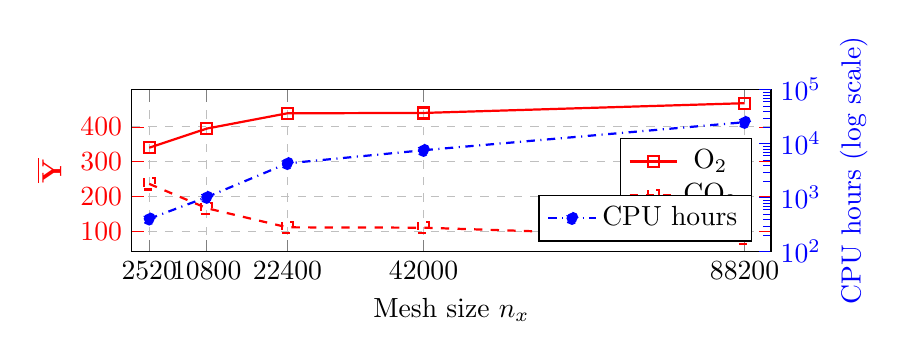
\begin{tikzpicture}
% First axis (left y-axis)
\begin{axis}[
    width=0.8\textwidth,
    height=0.3\textwidth,
    xlabel=Mesh size $n_x$,
    ylabel={\textcolor{red}{$\overline{\bY}$}},
    xmin=0, xmax=92000,
    xtick={2520,10800,22400,42000,88200},
    xticklabels={2520,10800,22400,42000,88200},
    ytick={100,200,300,400},
    ticklabel style={/pgf/number format/fixed},
    xmajorgrids=true,
    ymajorgrids=true,
    grid style=dashed,
    scaled ticks=false,
    legend style={at={(0.97,0.70)}, anchor=north east},
    ytick style={red},
    yticklabel style={red},
]
% O2 line (solid red)
\addplot[
    red,
    mark=square,
    thick
] coordinates {
    (2520,340)
    (10800,395)
    (22400,439)
    (42000,440)
    (88200,468)
}; 
% CO2 line (dashed red)
\addplot[
    red,
    mark=square,
    dashed,
    thick
] coordinates {
    (2520,236)
    (10800,166)
    (22400,111)
    (42000,110)
    (88200,80)
};
\legend{$\textnormal{O}_2$, $\textnormal{CO}_2$}
\end{axis}

% Second axis (right y-axis)
\begin{axis}[
    width=0.8\textwidth,
    height=0.3\textwidth,
    xmin=0, xmax=92000,
    ylabel={\textcolor{blue}{CPU hours (log scale)}},
    ymin=100, ymax=100000,
    ymode=log,
    axis x line=none,
    axis y line*=right,
    legend style={at={(0.97,0.35)}, anchor=north east},
    % y axis line style={blue},
    ytick style={blue},
    yticklabel style={blue},
]
\addplot[
    blue,
    dash dot,
    mark=*,
    thick
] coordinates {
    (2520,405)
    (10800,1020)
    (22400,4320)
    (42000,7560)
    (88200,25000)
};
\legend{CPU hours}
\end{axis}
\end{tikzpicture}

\caption{Convergence study. Mesh sizes $n_x \in \{2520, 10800, 22400, 42000, 88200\}$ are evaluated. The left y-axis corresponds to integrated mass fractions for $\textnormal{O}_2$ and $\textnormal{CO}_2$. The right y-axis corresponds to CPU hours on a logarithmic scale.}
\label{fig:convergence_study_plot}
\end{figure}


%%%%%%%%%%%%%%%%%%%%%%%% Operator Inference %%%%%%%%%%%%%%%%%%%%%%%
\section{Operator Inference reduced-order model with state constraints} \label{sec:OpInf_with_SL}
The char combustion model is governed by the gas phase conservation equations~\eqref{eq:gas_mass_conservation}--\eqref{eq:gas_energy_conservation}, the solid phase conservation equations~\eqref{eq:solid_mass_conservation}--\eqref{eq:solid_energy_conservation}, and the chemical reactions~\eqref{eq:heterogenous reaction}--\eqref{eq:homogeneous reaction}. However, similar to other legacy codes or commercial software, the complexity in the MFiX-PIC source code renders the derivation of high-fidelity operators associated with the nonlinear function $\bF$ in Eq.~\eqref{eq:general_nonlinear_ODE} impractical.
For exactly those settings, OpInf has emerged as an efficient scientific machine learning technique to construct predictive ROMs of high-dimensional dynamical systems. In particular, OpInf solely requires high-fidelity data to develop underlying low-fidelity models by learning polynomial ROMs. \par
In~\Cref{ss:data_pre_processing} and~\Cref{ss:dimensionality_reduction}, we present data pre-processing and dimension reduction techniques essential for constructing ROMs of multiphysics, multiscale applications.~\Cref{ss:OpInf_regularization} provides the theoretical background of the standard OpInf with regularization. In~\Cref{ss:species_limiter}, we introduce state constraints and their implementation details in the OpInf ROM. Also, we illustrate a stabilizing effect of state constraints, associated with the use of a global POD basis. 


%%%%%%%%%%%%%%%%%%%%%% Data-preprocessing %%%%%%%%%%%%%%%%%%%%%%%%%%%%
\subsection{Data pre-processing} \label{ss:data_pre_processing}
The variables in the training dataset encompass a broad range of numerical scales, as shown in~\Cref{tab:range_of_variable}. Specifically, pressure and temperature are on the orders of $10^5$ and $10^4$, respectively, whereas the mass fractions of certain species have magnitudes around $10^{-4}$. Such multiphysics and multiscale problems pose substantial challenges for model training, as larger magnitude variables can dominate those with smaller scales. To avoid numerical issues, it is advantageous to pre-process the FOM data to scale all variables to be in comparable orders of magnitude.
Firstly, the pressure and temperature, and their mean values, have relatively large magnitudes among all the variables considered. Thus, we center each pressure and temperature snapshot around zero via mean subtraction through 
\begin{align}
    \bq^{(\ell),{\textnormal{shifted}}}_{k} = \bq^{(\ell)}_{k} - \overline{\bq}^{(\ell)}, \hspace{2em} \overline{\bq}^{(\ell)} = \frac{1}{K} \sum_{k=0}^{K-1} \bq^{(\ell)}_{k}
\label{eq:shifting}
\end{align}
where $\ell$ indicates the state indices as in Eq.~\eqref{eq:l_th_state}, $\bq^{(l)}_{k} \in \real^{n_x}$ is the $k$th snapshot of the $\ell$th state, and $\overline{\bq}^{(\ell)} \in \real^{n_x}$ is its mean over $K$ snapshots. Note that we denote $\bQ^{(\ell), \textnormal{shifted}} \in \real^{n_x \times K}$ as the shifted snapshot matrix populated by $\bq^{(\ell),\textnormal{shifted}}_{k}$, where $k=0,1,\dots,K-1$.
However, the $x$, $y$, and $z$ velocities have relatively smaller magnitudes, with their means close to zero. Thus, we do not shift them. 
After shifting, if necessary, the pressure, temperature, and velocity snapshots are then scaled to ensure that all variables fall within the range of [$-1,1$]. We scale variables by dividing all elements by the maximum absolute value of the entire shifted matrix of each variable $\bQ^{(\ell),\textnormal{shifted}}$. The scaling process results in the scaled snapshot matrix of the $\ell$th variable as:
\begin{align}
    \bS^{(\ell)} = \frac{\bQ^{(\ell),{\textnormal{shifted}}}}{\textnormal{max}\left( | \bQ^{(\ell),\textnormal{shifted}} | \right)} \in \real^{n_x \times K}.
\label{eq:scaling}
\end{align}
Note that since the mass fractions fall within the interval [$0,1$], we do not pre-process them. Specifically, $\bS^{(\ell)} = \bQ^{(\ell)} \in \real^{n_x \times K}$ for snapshots of species mass fractions, where $\ell = 6$ corresponds to $\textnormal{O}_2$ mass fraction, $\ell = 7$ to $\textnormal{N}_2$ mass fraction, $\ell = 8$ to $\textnormal{CO}$ mass fraction, $\ell = 9$ to $\textnormal{CO}_2$ mass fraction, and $\ell = 10$ to $\textnormal{H}_2\textnormal{O}$ mass fraction.
After all pre-processing, the original training snapshot $\bQ \in \real^{N \times K}$ is transformed into the scaled snapshot $\bS \in \real^{N \times K}$.


%%%%%%%%%%%%%%%%%%%%%% Dimension reduction %%%%%%%%%%%%%%%%%%%%%%%%%%%%
\subsection{Dimensionality reduction} \label{ss:dimensionality_reduction}
Traditionally, OpInf adopts an approach in which snapshots of all state variables are aggregated, and subsequently, a global basis is derived via proper orthogonal decomposition (POD) from the comprehensive training snapshot matrix.
Although the authors in~\cite{benner2020operator2} used a block-diagonal projection matrix to address the topological structure of a highly coupled nonlinear problem, applying this method to our case led to poor prediction accuracy and a large ROM dimension due to the simulation of 10 physical variables.
Consequently---and for stability reasons outlined in~\Cref{ss:species_limiter}---we compute a global POD basis from the transformed snapshot matrix $\bS \in \mathbb{R}^{N \times K}$ of the stacked variables. The reduced singular value decomposition (SVD) of $\bS$, when $N \geq K$, is
\begin{equation}
    \bS = \bV \mathbf{\Sigma} \bW^{\top}
\label{eq:SVD}
\end{equation}
where the columns of $\bV \in \mathbb{R}^{N \times K}$ and  $\bW \in \real^{K \times K}$ are the left and right singular vectors of $\bS$, respectively. The singular values of $\bS$, denoted as $\sigma_1 \geq \sigma_2 \geq \cdots \geq \sigma_K \geq 0$, are on the diagonal of a diagonal matrix $\mathbf{\Sigma} \in \mathbb{R}^{K \times K}$. 
Note that the deterministic SVD of $\bS \in \real^{N \times K}$ has a complexity of \(O(N^2K + K^3)\), making it impractical due to the computational load that grows with the high degree-of-freedom $N$. Thus, we perform randomized SVD via the python package \texttt{Scikit-learn}~\cite{halko2011finding, pedregosa2018scikitlearnmachinelearningpython}.
The $r$ leading columns of the left singular vectors $\bV$ form the rank-$r$ linear POD basis as $\bV_r = [\bv_1, \dots, \bv_r] \in \real^{N \times r}$ whose each column is orthonormal, i.e., $\bV_r^\top \bV_r = \bI_r \in \real^{r \times r}$. We project the scaled snapshot matrix $\bS$ as
\begin{align}
    \widehat{\bS} = \bV_r^{\top}\bS=\left[ {\widehat{\bs}}_0 \hspace{0.7em} \cdots \hspace{0.7em} \widehat{\bs}_{K-1} \right] \in \mathbb{R}^{r \times K}.
\label{eq:low_dim_snapshots}
\end{align}
The full-order scaled state $\bs_k \in \real^{N}$ is approximated as $\bs_k \approx \bV_r \widehat{\bs}_k$. The low-dimensional snapshot matrix $\widehat{\bS}$ contains the data that are used to construct the ROM, which we describe next. 


%%%%%%%%%%%%%%%%%%%%%% OpInf with Regularization %%%%%%%%%%%%%%%%%%%%%%%%%%%%
\subsection{Operator Inference with regularization} \label{ss:OpInf_regularization}
OpInf learns the best-fit polynomial ROM from the projected data $\widehat{\bS}$ in Eq.~\eqref{eq:low_dim_snapshots}, potentially with added regularization or constraints. 
For the specific combustion problem considered in~\cite{jain2021performance}, including the cubic term in the right-hand side of the ROM provided a stabilizing effect. However, the number of entries in the reduced cubic operator scales with $r^4$, which needs to multiply with $r$ entries of the reduced state vector at every time step, resulting in the complexity of $r^5$ in an online ROM simulation.
Choosing a quadratic polynomial is often a good trade-off between model expressiveness and computational runtime for the ROM simulation~\cite{McQuarrie_2021, Swischuk_2020, qian2022reduced, farcas2023parametric, Zastrow2023, 0x003d183f, Rocha2023}. 
Thus, we opt to learn a quadratic OpInf model as
\begin{equation}
    \frac{\mathrm{d}\widehat{\bs}}{\mathrm{d}t} = \widehat{\bc} + \widehat{\bA} \widehat{\bs} + \widehat{\bH} \left( \widehat{\bs} \otimes \widehat{\bs} \right), \hspace{1.5em} t \in [t_0, t_{K-1}].
\label{eq:polynomial_ROM_eq}
\end{equation}
Here, the operator $\otimes$ indicates a compact Kronecker product that calculates the element-wise multiplication of two vectors while removing redundant quadratic terms. For example, when $\ba = [a_1, a_2, a_3]$, the compact Kronecker product is computed as $\ba \otimes \ba = [a_1^2, a_1a_2, a_1a_3, a_2^2, a_2a_3, a_3^2]$. 
The $\widehat{\bc} \in \real^r$ is a constant term, $\widehat{\bA} \in \real^{r \times r}$ is a linear operator, $\widehat{\bH} \in \mathbb{R}^{r \times r(r+1)/2}$ is a quadratic operator. \par

In the model learning process, it is crucial to avoid overfitting the quadratic model to the data due to potential noise or under-resolution of the data, the truncated global POD modes that result in unresolved system dynamics, and the potential for mis-specification of the ROM as fully quadratic, despite the highly nonlinear FOM encapsulated by the governing equations~\eqref{eq:gas_mass_conservation}--\eqref{eq:solid_energy_conservation}, and the chemical equations~\eqref{eq:heterogenous reaction}--\eqref{eq:homogeneous reaction}.
Therefore, we adopt Tikhonov regularization for OpInf, as in~\cite{McQuarrie_2021}.
The quadratic OpInf with regularization learns the reduced operators $\widehat{\bc}$, $\widehat{\bA}$, and $\widehat{\bH}$ in the least-squares problem
\begin{align}
    \min_{\widehat{\bc}, \widehat{\bA}, \widehat{\bH}} \quad & 
    \left\{ \sum_{k=0}^{K-1} \left\| \widehat{\mathbf{c}} + \widehat{\mathbf{A}} \widehat{\mathbf{s}}_k + \widehat{\mathbf{H}} \left( \widehat{\mathbf{s}}_k \otimes \widehat{\mathbf{s}}_k \right) - \dot{\widehat{\mathbf{s}}}_k \right\|_2^2 + \lambda_1 \left( \left\| \widehat{\mathbf{c}} \right\|_2^2 + \left\| \widehat{\mathbf{A}} \right\|_F^2 \right) + \lambda_2 \left\| \widehat{\mathbf{H}} \right\|_F^2 \right\} ,
\label{eq:optimization_regularized}
\end{align}
where $\widehat{\bs}_k \equiv \widehat{\bs}(t_k) $ represents the reduced state at the time step $k$. Note that the Kronecker product $\otimes$ introduces scaling differences between the entries of the quadratic operator $\widehat{\bH}$, and those in the constant operator $\widehat{\bc}$ and the linear operator $\widehat{\bA}$, when subjected to a single regularization parameter.
This motivates us to two regularization parameters $\lambda_1 > 0$ and $\lambda_2 > 0$, such that $\lambda_1$ penalizes $\widehat{\bc}$ and $\widehat{\bA}$, and $\lambda_2$ penalizes $\widehat{\bH}$.
The $\dot{\widehat{\bs}}_k \equiv \dot{\widehat{\bs}}(t_k)$ denotes the time derivative of the reduced state at the time step $k$, and it can be computed using a suitable time derivative approximation scheme. We use a $6$th-order central finite difference method, with biased forward and backward differencing applied at the initial and final time steps.
Equation~\eqref{eq:optimization_regularized} can be written compactly as
\begin{align}
    \min_{\bO} \left\| \mathbf{DO}^{\top} - \dot{\widehat{\bS}}^{\top} \right\|_{F}^{2} + \left\|\mathbf{\Lambda} \bO^{\top} \right\|_{F}^{2}, \quad \text{where} \quad
    \bO = \left[\widehat{\bc} \hspace{0.7em} \widehat{\bA} \hspace{0.7em} \widehat{\bH} \right], \hspace{0.7em}
    \bD = \left[\mathbf{1}_K \hspace{0.5em} \widehat{\bS}^{\top} \hspace{0.5em} \left(\widehat{\bS} \otimes \widehat{\bS} \right)^{\top} \right],
\label{eq:regularization_matrix_form}
\end{align}
and where $\bO \in \mathbb{R}^{r \times d(r)}$ and $\bD \in \mathbb{R}^{K \times d(r)}$.
Here, $\dot{\widehat{\bS}} \in \real^{r \times K}$ is a matrix whose columns are $\dot{\widehat{\bs}}_k$, and $\mathbf{1}_K \in \mathbb{R}^K$ is a column vector of length $K$ with all entries set to one. Also, $\mathbf{\Lambda} = \textnormal{diag}(\lambda_1, \lambda_1 \bI_{r}, \lambda_2 \bI_{r(r+1)/2}) \in \mathbb{R}^{d(r) \times d(r)}$ serves as a diagonal regularization matrix, where $\bI_{r}$ and $\bI_{r(r+1)/2}$ are identity matrices with dimensions $r$ and $r(r+1)/2$, respectively, making $d(r) = 1+r+r(r+1)/2$. In practice, we must carefully choose the regularization parameters $\lambda_1$ and $\lambda_2$; see~\Cref{ss:regularization_hyperparameters_selection} for details. 
The reduced operators inferred by solving Eq.~\eqref{eq:regularization_matrix_form} provide the best fits of reduced state trajectories of the ROM Eq.~\eqref{eq:polynomial_ROM_eq} within the training regime in a minimum residual sense.



%%%%%%%%%%%%%%%%%%%%%% State constraints %%%%%%%%%%%%%%%%%%%%%%%%%%%%
\subsection{State constraints to enforce physical consistency of the operator inference reduced-order model} \label{ss:species_limiter}
Low-dimensional surrogate modeling is challenging for nonlinear multiscale and multiphysics problems. Consequently, there have been many research advances to ensure better predictive capabilities of these models.
As previously discussed in~\Cref{sec:intro}, various structure-preserving methods offer an approach to enforce physical consistency in OpInf ROMs. While these approaches have successfully addressed issues of mathematical stability, energy preservation, and conservation of mechanistic principles, they are not guaranteed to provide ROM predictions that are consistent with the physical constraints inherent in the FOM.
In this section, we propose a method for maintaining these intrinsic physical constraints within the state prediction via OpInf ROMs.
Specifically, we build on an idea proposed in~\cite{huang2020species}---embedding species limiters as the state constraints for intrusive projection-based ROMs for combustion reacting flows---into the state prediction process via operator-inferred ROMs.

\subsubsection{Limitation of the standard operator inference reduced-order model} \label{sss:Outline_state_constrained_OpInf}
~\Cref{fig:species_limiter_step} highlights the contrast in state propagation when using standard OpInf compared to the proposed scheme with state constraints. The standard OpInf propagates states only in the low-dimensional space from the initial reduced state $\widehat{\bs}_0$ to the final reduced state $\widehat{\bs}_{K_f-1}$ through a numerical time integration. Here, $K_f$ represents the total number of snapshots forecasted through OpInf beyond the training regime.~Once the temporal evolution of all the reduced states $\widehat{\bs}_k$ is done, the high-dimensional states are reconstructed by $\widetilde{\bS} = \bV_r \widehat{\bS} \in \real^{N \times K_f}$. 
However, the reconstructed high-dimensional state $\widetilde{\bs}_k$ is not guaranteed to comply with the potential physical constraints posed by the physics of the FOM.
Particularly for the char combustion data considered herein, some predicted species mass fractions, which are in $\widetilde{\bS}^{(\ell)}$, where $\ell=6,7,8,9,10$ as discussed in~\Cref{ss:data_pre_processing}, may not fall within the range $[0,1]$. In fact, even the reconstruction of the initial reduced state, which is $\bV_r \widehat{\bs}_0$, is not assured to provide mass fractions consistent with such a constraint.

\subsubsection{Design of state constraints}     \label{sss:design_state_constraints}
In the proposed framework of OpInf ROM with state constraints, we enforce the state constraints to the reconstructed high-dimensional state $\widetilde{\bs}_k \in \real^{N}$ at every time step during the state propagation. Since the available FOM data of the char combustion does not provide sufficient information to determine whether pressure, temperature, and velocities inherit physical constraints, we limit our state constraints to the species mass fraction variables. This is problem-specific; thus, if physical limitations regarding other variables are available from prior knowledge of the FOM, different constraints may have to be applied.
By embedding state constraints for the species mass fraction variables, we aim to enhance the physical consistency of the predictions made by the OpInf ROM, thereby improving its ability to stably and accurately capture the complex dynamics of char combustion processes while maintaining computational efficiency. \par


% Define custom colors
\definecolor{C00}{rgb}{0.121, 0.467, 0.705} % skyblue
\definecolor{C01}{rgb}{1.000, 0.498, 0.055} % Orange
\definecolor{C02}{rgb}{0.172, 0.627, 0.173} % Green
\definecolor{C03}{rgb}{0.839, 0.153, 0.157} % red
\definecolor{C04}{rgb}{0.580, 0.404, 0.741} % purple
\definecolor{C05}{rgb}{0.549, 0.337, 0.294} % brown
\definecolor{C06}{rgb}{0.890, 0.467, 0.761} % pink
\definecolor{C07}{rgb}{0.498, 0.498, 0.498} % gray
\definecolor{C08}{rgb}{0.737, 0.741, 0.133} % yellow
\definecolor{C09}{rgb}{0.090, 0.745, 0.812} % cyan


%% state-constraints steps %%
\begin{figure}[H]
    \centering
    \begin{tikzpicture}[
        node distance=1.0cm and 1.0cm,
        every node/.style={align=center},
        lowdim/.style={font=\small},
        highdim/.style={font=\small},
        vec/.style={->, thick, C02},
        sl/.style={->, thick, C02},
        transform/.style={->, thick, C02},
        reduction/.style={->, thick, C02},
    ]
    
    % Low-dimensional nodes
    \node[lowdim] (s0) {$\widehat{\bs}_0$};
    \node[lowdim, right=of s0] (s0*) {$\widehat{\bs}_0^{*}$};
    \node[lowdim, right=of s0*] (s1) {$\widehat{\bs}_1$};
    \node[lowdim, right=of s1] (s1*) {$\widehat{\bs}_1^{*}$};
    \node[lowdim, right=of s1*] (s2) {$\widehat{\bs}_2$};
    \node[lowdim, right=of s2] (s2*) {$\widehat{\bs}_2^{*}$};
    \node[lowdim, right=of s2*] (s3) {$\widehat{\bs}_3$};
    
    \node[lowdim, right=0.1cm of s3] (dots) {$\cdots$};
    
    % High-dimensional nodes
    \node[highdim, below=of s0] (S0) {$\widetilde{\bs}_0$};
    \node[highdim, right=of S0] (S0*) {$\widetilde{\bs}_0^*$};
    \node[highdim, below=of s1] (S1) {$\widetilde{\bs}_1$};
    \node[highdim, right=of S1] (S1*) {$\widetilde{\bs}_1^*$};
    \node[highdim, below=of s2] (S2) {$\widetilde{\bs}_2$};
    \node[highdim, right=of S2] (S2*) {$\widetilde{\bs}_2^*$};

    % Horizontal arrows for low-dimensional row
    \draw[vec] (s0*) -- node[midway,above] {\textcolor{C02}{ROM}} (s1);
    \draw[vec] (s1*) -- node[midway,above] {\textcolor{C02}{ROM}} (s2);
    \draw[vec] (s2*) -- node[midway,above] {\textcolor{C02}{ROM}} (s3);

    % Normal ROM state propagation
    \draw[C01, thick, dashed, ->, bend left=65] (s0) to node[midway,above,sloped] {ROM} (s1);
    \draw[C01, thick, dashed, ->, bend left=65] (s1) to node[midway,above,sloped] {ROM} (s2);
    \draw[C01, thick, dashed, ->, bend left=65] (s2) to node[midway,above,sloped] {ROM} (s3);

    % Arrows between high-dim and stabilized high-dim
    \draw[sl] (S0) -- node[midway,below] {species \\ limiters} (S0*);
    \draw[sl] (S1) -- node[midway,below] {species \\ limiters} (S1*);
    \draw[sl] (S2) -- node[midway,below] {species \\ limiters} (S2*);
    
    % Arrows between low-dim and high-dim
    \draw[transform] (s0) -- node[midway,right] {$\bV_r \times$} (S0);
    \draw[transform] (s1) -- node[midway,right] {$\bV_r \times$} (S1);
    \draw[transform] (s2) -- node[midway,right] {$\bV_r \times$} (S2);
    
    % Arrows between stabilized high-dim and low-dim
    \draw[reduction] (S0*) -- node[midway,right] {$\bV_r^{\top} \times$} (s0*);
    \draw[reduction] (S1*) -- node[midway,right] {$\bV_r^{\top} \times$} (s1*);
    \draw[reduction] (S2*) -- node[midway,right] {$\bV_r^{\top} \times$} (s2*);
    
    \node[left=of s0] {\\ Low-dimensional \\ space};
    \node[left=of S0] {\\ High-dimensional \\ space};

    \usetikzlibrary{calc}
    \usetikzlibrary{backgrounds}
    \pgfdeclarelayer{background}
    \pgfsetlayers{background,main}
    \begin{scope}[on background layer]
        \draw[solid, thick, black]
            ($(s0.north west)+(-4.2cm, 1.5cm)$) rectangle 
            ($(S2*.south east)+(2.9cm,-0.9cm)$);
    \end{scope}
    
    \end{tikzpicture}
    \caption{Schematic of the state propagation in the ROM with species limiters, which are state constraints for the species mass fractions. The dashed arrows represent the reduced state propagation via the standard OpInf ROM, and the solid arrows represent the state propagation via the OpInf with species limiters. The orthogonal basis $\bV_r \in \real^{N \times r}$ is used for projection between the low-dimensional space $\real^{r}$ and the high-dimensional space $\real^{N}$.}
    \label{fig:species_limiter_step}
\end{figure}

To design state constraints on species mass fractions, we use the knowledge of the variable ranges as well as boundary conditions of the FOM, as shown in~\Cref{tab:combustion_parameters}, and chemical reactions~\eqref{eq:heterogenous reaction}--\eqref{eq:homogeneous reaction}. 
Concerning the air inflow boundary conditions of the combustion model, the maximum permissible values of the mass fractions of $\textnormal{O}_2$, $\textnormal{N}_2$, and $\textnormal{H}_2\textnormal{O}$ are dictated by the corresponding constituents within the air inflow, given that these components are not produced from both Eqs.~\eqref{eq:heterogenous reaction}--\eqref{eq:homogeneous reaction}. The $\textnormal{CO}$ and $\textnormal{CO}_2$ do not constitute the inlet air inflow and are the products of the two chemical reactions considered. Thus, we can only set their upper limits to $1$, the possible maximum value of species mass fractions.
Moreover, all species must have non-negative mass fractions, establishing a lower limit of $0$. However, we introduce a very small uniform random noise $Z$ to account for the highly oscillatory behavior of mass fractions observed in the FOM data. 
In sum, we formulate the state constraints of all species mass fractions as
\begin{align} 
    \label{eq:species_limiter_O2}
    Y_{\textnormal{O}_2} &\leftarrow \max \left( \min \left( Y_{\textnormal{O}_2}, 0.23 \right), Z \right) \\
    \label{eq:species_limiter_N2}
    Y_{\textnormal{N}_2} &\leftarrow \max \left( \min \left( Y_{\textnormal{N}_2}, 0.76 \right), Z \right) \\
    \label{eq:species_limiter_CO}
    Y_{\textnormal{CO}} &\leftarrow \max \left( \min \left( Y_{\textnormal{CO}}, 1.00 \right), Z \right) \\
    \label{eq:species_limiter_CO2}
    Y_{\textnormal{CO}_2} &\leftarrow \max \left( \min \left( Y_{\textnormal{CO}_2}, 1.00 \right), Z \right) \\
    \label{eq:species_limiter_H2O}
    Y_{\textnormal{H}_2\textnormal{O}} &\leftarrow \max \left( \min \left( Y_{\textnormal{H}_2\textnormal{O}}, 0.10 \right), Z \right)
\end{align}
where $Z \sim U(\kappa_1,\kappa_2)$ represents a random variable uniformly distributed over the interval [$\kappa_1,\kappa_2$]. In our case, $\kappa_1 = 10^{-10}$ and $\kappa_2 = 10^{-5}$ are used. \par

\subsubsection{ROM state propagation with state constraints} \label{sss:state_propagation_state_constraints}
In~\Cref{fig:species_limiter_step}, we illustrate that states propagate across two spaces within the OpInf ROM with species limiters.
To maintain the physical consistency from the initial time step, the initial reduced state $\widehat{\bs}_0$ first must be lifted to high-dimensional state $\widetilde{\bs}_0$ that contains all variables.
The state constraints, formulated as Eqs.~\eqref{eq:species_limiter_O2}--\eqref{eq:species_limiter_H2O}, are directly enforced to $\widetilde{\bs}_0$, leading to the modified high-dimensional state $\widetilde{\bs}_0^*$. This subsequently needs to be projected back to $\widehat{\bs}^*_0$, so that the ROM propagates $\widehat{\bs}_0^*$ to $\widehat{\bs}_1$. In this manner, we propagate states over time within the low-dimensional space, thereby maintaining computational efficiency. This iterative procedure continues until the final time.
Once the entire temporal propagation is done, we unscale the modified high-dimensional states $\widetilde{\bs}^*_k$ ($k=0,1,\ldots,K_f-1$), which contain scaled variables such as pressure, temperature, and velocities, via the inversion of Eqs.~\eqref{eq:shifting}--\eqref{eq:scaling}, obtaining the high-dimensional states in the original scale $\widetilde{\bq}^*_k$.
Note that since we only constrain the species mass fraction variables, which are not scaled initially, we obviate the necessity to restore the original scales of $\widetilde{\bs}_k$ at every time step during the state propagation. Nevertheless, should limiting conditions pertain to pre-processed variables, restoring their original scales in the high-dimensional space becomes necessary at each time step prior to enforcing state constraints.
~\Cref{al:OpInf_with_SL} provides the algorithmic process of OpInf with species limiters. Note that the model learning process, including data pre-processing, SVD, and regularization, requires $K$ training snapshots, and the temporal propagation with state constraints can go beyond this training regime, to $K_f$ time steps.
%%%%%%%%%%%%%%%%%%%%%% Algorithm %%%%%%%%%%%%%%%%%%%%%%%%
\begin{algorithm}
\caption{Operator Inference with species limiters}  \label{al:OpInf_with_SL}
\begin{algorithmic}[1]
    \Procedure{OpInf with species limiters}{}
    
    \State Transform original snapshots $\bQ \in \real^{N \times K}$ into $\bS \in \real^{N \times K}$ as in Eqs.~\eqref{eq:shifting}--\eqref{eq:scaling}
    
    \State Compute randomized SVD with a target rank $r_t$:
    $\bS = \bV_{r_t} \mathbf{\Sigma}_{r_t} \bW_{r_t}^{\top}$ where $\bV_{r_t} \in \real^{N \times r_t}$, $\mathbf{\Sigma}_{r_t} \in \real^{{r_t} \times {r_t}}$, and $\bW_{r_t} \in \real^{K \times {r_t}}$

    \State Select a rank-$r$ low-dimensional basis $\bV_r = \bV_{r_t}[:,:r]$
    
    \State Project $\bS$ to the linear low-dimensional subspace: $\widehat{\bS} = \bV_r^{\top} \bS \in \real^{r \times K}$

    \State Evaluate the time derivative of the reduced snapshot $\widehat{\bS}$

    \Procedure{Regularization}{}
    
    \State Search hyperparameters $\lambda_1^{*}$ and $\lambda_2^{*}$ based on the key performance indicator criterion as in Eq.~\eqref{eq:thermal_energy_eq}
    
    \EndProcedure
    
    \Procedure{Time propagation over $K_f$ time steps with species limiters}{}
    \For{$k=0, \dots, K_f-1$}
        \State Reconstruct the high-dimensional state: $\widetilde{\bs}_{k} = \bV_r \widehat{\bs}_k \in \real^{N}$
        
        \State Apply the species limiters Eqs.~\eqref{eq:species_limiter_O2}--\eqref{eq:species_limiter_H2O}, to $\widetilde{\bs}_k$, obtaining a modified full-state $\widetilde{\bs}_k^*$

        \State Project $\widetilde{\bs}_k^{*}$ to the low-dimensional subspace: $\widehat{\bs}_k^{*} = \bV_r^{\top} \widetilde{\bs}_k^{*}$

        \State Propagate from $\widehat{\bs}_k^{*}$ to $\widehat{\bs}_{k+1}$ by time integration of Eq.~\eqref{eq:polynomial_ROM_eq}

    \EndFor
    \EndProcedure

    \State Restore high-dimensional states $\widetilde{\bq}_{k}^{*}$ in the original scales from $\widetilde{\bs}_{k}^{*}$
    
    \State \Return $\bQ^{*} = [ \widetilde{\bq}_0^{*} \hspace{1em} \widetilde{\bq}_1^{*} \hspace{1em} \cdots \hspace{1em} \widetilde{\bq}_{K_f-1}^{*} ] \in \real^{N \times K_f}$
\EndProcedure
\end{algorithmic}
\end{algorithm}


%%%%%%%%%%%%%%%%%%%%%% Stabilizing effect %%%%%%%%%%%%%%%%%%%%%%%%%%%%
\subsubsection{Stabilizing effect of ROM with state constraints} \label{sss:stabilizing_effect}
The species limiters that act on a part of the state indeed have a stabilizing effect on the entire state vector, and the global POD basis plays a crucial role in it.~\Cref{fig:state_correction_illustration} provides a graphical understanding of the state propagation, embedded with state constraints.
\begin{figure}[htbp]
\centering
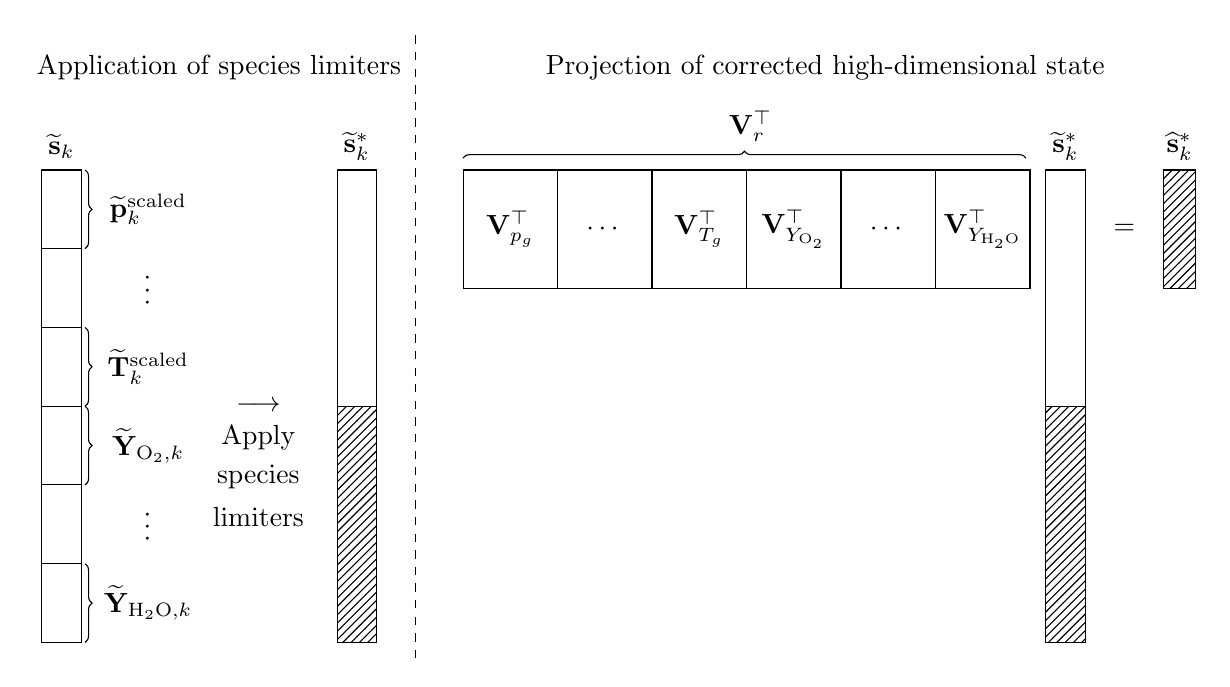
\begin{tikzpicture}[
    box/.style={draw, minimum width=1.2cm, minimum height=1.5cm, inner sep=0pt},
    box2/.style={draw, minimum width=1.5cm, minimum height=1.0cm, inner sep=0pt},
    short vec/.style={draw, minimum width=0.4cm, minimum height=1.5cm, inner sep=0pt},
    long vec/.style={draw, minimum width=0.5cm, minimum height=6cm, inner sep=0pt},
    short var/.style={draw, minimum width=0.5cm, minimum height=1.0cm, inner sep=0pt},
    hatched long box/.style={draw, pattern=north east lines, minimum width=0.5cm, minimum height=3.0cm, inner sep=0pt},
    hatched short box/.style={draw, pattern=north east lines, minimum width=0.4cm, minimum height=1.5cm, inner sep=0pt}
]
    \draw (-13, 7.2) node[long vec] {};
    \node at (-13, 10.5) {$\widetilde{\bs}_k$};

    \draw (-13, 9.7) node[short var] {};
    \draw (-13, 8.7) node[short var] {};
    \draw (-13, 7.7) node[short var] {};
    
    \draw (-13, 6.7) node[short var] {};
    \draw (-13, 5.7) node[short var] {};
    \draw (-13, 4.7) node[short var] {};

    \draw[decorate,decoration={brace}] (-12.7, 10.2) -- (-12.7, 9.2);
    \node at (-11.9, 9.7) {$\widetilde{\bp}^{\textnormal{scaled}}_k$};
    \node[rotate=90] at (-11.9, 8.7) {$\cdots$};
    \draw[decorate,decoration={brace}] (-12.7, 8.2) -- (-12.7, 7.2);
    \node at (-11.9, 7.7) {$\widetilde{\bT}^{\textnormal{scaled}}_k$};
    \draw[decorate,decoration={brace}] (-12.7, 7.2) -- (-12.7, 6.2);
    \node at (-11.9, 6.7) {$\widetilde{\bY}_{\textnormal{O}_2,k}$};
    \node[rotate=90] at (-11.9, 5.7) {$\cdots$};
    \draw[decorate,decoration={brace}] (-12.7, 5.2) -- (-12.7, 4.2);
    \node at (-11.9, 4.7) {$\widetilde{\bY}_{\textnormal{H}_2\textnormal{O},k}$};
    
    \node at (-10.5, 7.2) {$\longrightarrow$};

    \node at (-10.5, 6.8) {Apply};
    \node at (-10.5, 6.3) {species};
    \node at (-10.5, 5.8) {limiters};

    \draw (-9.25, 7.2) node[long vec] {};
    \node at (-9.25, 10.5) {$\widetilde{\bs}_k^*$};

    \usetikzlibrary{patterns}
    \draw (-9.25, 5.7) node[hatched long box] {};

    \draw[dashed] (-8.5, 4) -- (-8.5, 12);

    \node at (-11, 11.5) {\text{Application of species limiters}};

    \foreach \x in {1.2, 2.4, 3.6, 4.8, 6.0, 7.2} {
        \draw (-8.50+\x, 9.45) node[box] {};
    }
    \node at (-7.3, 9.45) {$\bV_{p_g}^\top$};
    \node at (-6.1, 9.45) {$\cdots$};
    \node at (-4.9, 9.45) {$\bV_{T_g}^\top$};
    \node at (-3.7, 9.45) {$\bV_{Y_{\textnormal{O}_2}}^\top$};
    \node at (-2.5, 9.45) {$\cdots$};
    \node at (-1.3, 9.45) {$\bV_{Y_{\textnormal{H}_2\textnormal{O}}}^\top$};

    \node at (-4.25, 10.75) {$\bV_r^\top$};
    \draw[decorate,decoration={brace}] (-7.90, 10.35) -- (-0.75, 10.35);

    \draw (-0.25, 7.2) node[long vec] {};
    \node at (-0.25, 10.5) {$\widetilde{\bs}_k^*$};

    \usetikzlibrary{patterns}
    \draw (-0.25, 5.7) node[hatched long box] {};
    
    \node at (0.5, 9.45) {=};

    \draw (1.2, 9.45) node[hatched short box] {};
    \node at (1.2, 10.5) {$\widehat{\bs}_k^*$};

    \node at (-3.3, 11.5) {\text{Projection of corrected high-dimensional state}};
\end{tikzpicture}
\caption{Interpretation of the state constraints-embedded state propagation, as presented in ~\Cref{fig:species_limiter_step}. The process is illustrated for a single time step. The left-hand side of the vertical dotted line represents the enforcement of species limiters, and the shaded area of $\widetilde{\bs}_k^*$ represents the modified values. The right-hand side of the vertical dotted line represents the projection of the partially modified high-dimensional state, modifying all the entries of the reduced state $\widehat{\bs}_k^*$.}
\label{fig:state_correction_illustration}
\end{figure}
Since we use the global POD basis computed from stacked state snapshots, see \Cref{ss:dimensionality_reduction}, the linear combination of the $r$ columns of $\bV_{r}[(\ell-1)n_x:\ell n_x - 1, :] \in \real^{n_x \times r}$ and the $r$ entries of $\widetilde{\bs}_k$ reconstructs each $\ell$th state vector, which is denoted as $\widetilde{\bs}_k[(\ell-1)n_x:\ell n_x - 1]$. For example, the reconstructed scaled pressure vector at time step $k$, $\widetilde{\bp}_k^{\textnormal{scaled}} \in \real^{n_x}$, is computed as a linear combination of the columns of $\bV_{p_g}$ and the entries of $\widehat{\bs}_k$, where $\bV_{p_g}$ is the first $n_x$ rows of the global basis $\bV_r \in \real^{N \times r}$. In other words, when $\bV_{p_g} = \left[ \bv_{p_g,1}, \cdots, \bv_{p_g,r} \right] \in \real^{n_x \times r}$, $\widetilde{\bp}_k^{\textnormal{scaled}}$ is computed as $\sum_{\eta=1}^{r} \widehat{\bs}_{k,\eta} \cdot \bv_{p_g,\eta}$.
After all the states are reconstructed, leading to $\widetilde{\bs}_k$, we enforce the state constraints to the mass fraction states. Thus, $\widetilde{\bY}_{\textnormal{O}_2, k}$, $\widetilde{\bY}_{\textnormal{N}_2, k}$, $\widetilde{\bY}_{\textnormal{CO}, k}$, $\widetilde{\bY}_{\textnormal{CO}_2, k}$, and $\widetilde{\bY}_{\textnormal{H}_2\textnormal{O}, k}$ are corrected, producing a modified high-dimensional state $\widetilde{\bs}_k^*$. In \Cref{fig:state_correction_illustration}, we indicate the modified states with a shaded area.
Afterward, we compress $\widetilde{\bs}_k^*$ through the global POD basis $\bV_r$, resulting in the low-dimensional state $\widehat{\bs}_k^*$. We can view the numerical aspect of this projection in two ways. First, it is a linear combination of all the columns of $\bV_r^\top$ and all the entries of $\widetilde{\bs}_k^*$, meaning $\widehat{\bs}_k^* = \sum_{n=1}^{N} \widetilde{\bs}^{*}_{k,n} \cdot \bV_r^\top[:,n]$.
Another is that each entry of $\widehat{\bs}_k^*$, denoted as $\widehat{\bs}^{*}_{k,\eta}$ ($\eta = 1,2,\cdots,r$), is the outer product between a row vector of $\bV_r^\top$, which is $\bV_r^\top[\eta,:]$, and a column vector $\widetilde{\bs}^*_{k}$. Either way, all the entries of the resultant low-dimensional state $\widehat{\bs}_k^*$ are modified. Note that the ROM propagates the reduced states with all the entries changed. Thus, in the next time step $k+1$, the trajectories of the reconstructed high-dimensional states that are not subject to any constraints also change due to the species limiters. In our case, this provided stabilizing effects on the entire state variables, as further shown in the numerical results in \Cref{sss:results}. 
We also investigate the use of a block-structured, rather than a stacked, POD basis; however, this produces poor accuracy with the dataset considered herein. Further, we illustrate in~\ref{app:block_POD} that a block-structured projection matrix may not have the same global stabilizing effect on all variables. 

%%%%%%%%%%%%%%%%%%%%%%%%%%%% Numerical results %%%%%%%%%%%%%%%%%%%%%%%%%%%%%%%%
\section{Numerical results} \label{sec:numerical_results}
This section presents the numerical results of our study on OpInf ROMs with state constraints for the char combustion problem.
\Cref{ss:FOM_data_set} presents the details of the MFiX-PIC FOM data from which the ROM is constructed.
In \Cref{ss:basis_selection}, we discuss the ROM dimension selection process.
\Cref{ss:regularization_hyperparameters_selection} presents the regularization hyperparameters selection process, where we propose a new selection criterion via a key performance indicator.
In \Cref{ss:various_methods}, we analyze the effect of enforcing state constraints to OpInf on stability, accuracy, and computational efficiency by comparing it with standard OpInf and other stability-enhancing OpInf approaches. 


%%%%%%%%%%%%%%%%%%%%%%%%%%%% FOM data set %%%%%%%%%%%%%%%%%%%%%%%%%%%%%%%%
\subsection{FOM data details}    \label{ss:FOM_data_set}
The training data generated by MFiX-PIC consist of solution variables from Eq.~\eqref{eq:solution_variables} over $n_x = 22{,}400$ cells, with $N = n_v \times n_x = 224{,}000$ being the degrees of freedom of the high-fidelity system. The FOM simulation generates snapshots over 38 seconds (from 2 to 40 seconds) with an adaptive time step ranging from $10^{-8}$s to $10^{-4}$s. The snapshots are saved every $\delta t=10^{-3}s$, providing $K_f=38{,}000$ snapshots, where the initial $K=12{,}000$ snapshots (32\%) are used for training, and the remaining $26{,}000$ snapshots (68\%) are used for testing. In other words, our testing interval goes 200\% beyond the training interval. The high-dimensional data generation took approximately 56 days with an MPI-based solver on 45 CPUs, corresponding to 60,480 CPU hours (Intel Xeon W-3175X CPU @ 3.10 GHz). 
The construction of the OpInf ROM utilizes the training snapshot matrix $\bQ \in \real^{224{,}000 \times 12{,}000}$.~\Cref{tab:range_of_variable} shows the range of state variables within the training regime, which is essential for the data pre-processing step, as elaborated in~\Cref{ss:data_pre_processing}.
\begin{table}[H]
    \centering
    \caption{The minimum, mean, and maximum values of state variables within the MFiX-PIC training dataset. The solutions on the $22{,}400$ cells over $12{,}000$ snapshots are considered for all $n_v = 10$ state variables.}
    \vspace{-1em}
    \begin{tabular}{r|r r r r r}
    Variable   & Minimum   & Mean   & Maximum   \\ \hline
    Pressure [$\textnormal{Pa}$] & $9.876 \times 10^4$ & $1.014 \times 10^5$ & $2.600\times10^5$   \\ 
    x velocity [$\textnormal{m/s}$] & $-1.752\times10$ & $2.203 \times 10^{-4}$ & $1.742 \times 10$  \\ 
    y velocity [$\textnormal{m/s}$] & $-2.752\times10$ & $-9.470 \times 10^{-1}$ & $1.261 \times 10$  \\ 
    z velocity [$\textnormal{m/s}$] & $-1.507\times10$ & $1.888\times10^{-4}$ & $1.542 \times 10$ \\ 
    Temperature [$\textnormal{K}$] & $5.748\times10^2$ & $1.133\times10^3$ & $2.361\times10^4$ \\ 
    $\textnormal{O}_2$ mass fraction  & $0$ & $1.756\times10^{-1}$ & $2.300\times10^{-1}$  \\ 
    $\textnormal{N}_2$ mass fraction & $2.166\times10^{-1}$ & $7.455\times10^{-1}$ & $7.600\times10^{-1}$  \\ 
    $\textnormal{CO}$ mass fraction & $0$ & $8.933\times10^{-4}$ & $7.507\times10^{-1}$ \\ 
    $\textnormal{CO}_2$ mass fraction & $0$ & $6.820\times10^{-2}$ & $3.799\times10^{-1}$ \\ 
    $\textnormal{H}_2\textnormal{O}$ mass fraction & $2.851\times10^{-3}$ & $9.810\times10^{-3}$ & $1.000\times10^{-2}$
    \end{tabular}
    \label{tab:range_of_variable}
\end{table}


%%%%%%%%%%%%%%%%%%%%%% ROM dimension selection %%%%%%%%%%%%%%%%%%%%%%%%%%%
\subsection{Selection of the ROM dimension}    \label{ss:basis_selection}
Conventionally, POD considers an energy metric to determine the ROM dimension $r$. The cumulative energy $\cE_{\text{cum}}(r)$ is defined as the ratio of the sum of squared singular values up to rank $r$ to the total sum of squared singular values: $\cE_{\text{cum}}(r) =\sum_{\eta=1}^{r}\sigma_{\eta}^2 / \sum_{\eta=1}^{r_t}\sigma_{\eta}^{2}$, where the $\sigma_{\eta}$ ($\eta=1,2,\dots,r_t$) are the singular values of the scaled snapshot matrix $\bS$. Here, $r_t$ is the number of singular values to extract when we use randomized SVD in practice. This cumulative energy connects the low-rank dimension $r$ to the relative projection error of the scaled snapshot $\bS$ as
\begin{equation}
    \cE_{\text{proj}}(r) = \frac{\left\| \bS - \bV_r \bV_r^{\top} \bS \right\|_F^2}{\left\| \bS \right\|_F^2} = 1 - \cE_{\text{cum}}(r).
\label{eq:energy_criterion}
\end{equation}
For this data set, we found that $\cE_{\textnormal{proj}}(1) = 0.005$, meaning the cumulative energy is $0.995$ with $r=1$. Despite the first mode containing most of the system energy, choosing only one global mode for all variables is insufficient to capture the complex dynamics and sensitivities of the combustion model. \par

Instead of evaluating the single projection error of the scaled snapshot matrix $\bS$ that contains all the scaled variables, we can also calculate the projection error for each variable in its original scales, with respect to the low-dimensional rank-$r$ basis $\bV_r$. This involves reconstructing the scaled snapshots as $\widetilde{\bS} = \bV_r \bV_r^\top \bS$, followed by restoring the original scales of all $n_v = 10$ variables through the inversion of Eqs.~\eqref{eq:shifting}--\eqref{eq:scaling}. Denoting the reconstructed snapshot matrix of the $\ell$th state in its original scale as $\widetilde{\bQ}^{(\ell)} \in \real^{n_x \times K}$ (see \Cref{ss:data_pre_processing} for notation), the relative error is computed with respect to the true $\ell$th state snapshot matrix $\bQ^{(\ell)} \in \real^{n_x \times K}$.
 \begin{figure}[ht]
    \centering
    \includegraphics[width=1.0\textwidth]{figures/snapshot_proj_error.png}
    \vspace{-1.5em}
    \caption{Projection errors of each variable. The errors are computed with the variables in their original scales as $ \| \bQ^{(\ell)} - \widetilde{\bQ}^{(\ell)} \|_F^{2} / \| \bQ^{(\ell)} \|_F^{2}$. }
    \label{fig:projection_error_all}
\end{figure}    
~\Cref{fig:projection_error_all} shows the variable-specific projection errors in their original scales with respect to the low-rank dimension $r$. Pressure, $\textnormal{N}_2$, and $\textnormal{H}_2\textnormal{O}$ mass fractions exhibit notably low errors, in turn indicating high energy capture. Conversely, $\textnormal{CO}$ mass fraction and velocity components ($v_x$, $v_y$, $v_z$) display higher errors. This discrepancy is in part due to their relatively small scales, which skew the errors when considered in the denominator of the relative error metric. These observations highlight the strong dependence of projection errors on the specific variable under consideration. This variability suggests that the effectiveness of the rank-$r$ basis in capturing the system's dynamics is not uniform across all variables. \par

In conclusion, neither the projection error of the individual variables nor the energy associated with the entire scaled snapshot matrix $\bS$ provides a comprehensive representation of the complex and multiscale characteristics of this dataset.
After several tests, we select $r=30$ because it reasonably captures the high-frequency fluctuating dynamics of the FOM while providing a manageable model dimension. 
For this dataset, selecting more than $30$ modes is ineffective. This is because the regularization hyperparameter selection process, which is discussed next, substantially increases the computational time.



%%%%%%%%%%%%%%%%%%%%%% Regulariztion hyperparameters selection %%%%%%%%%%%%%%%%%%%%%%%%%%%
\subsection{Regularization hyperparameters selection based on key performance indicator}    \label{ss:regularization_hyperparameters_selection}
To select the hyperparameters $\lambda_1$ and $\lambda_2$ for regularizing the least-squares problem in Eq.~\eqref{eq:optimization_regularized}, we create a logarithmically-spaced uniform parameter grid, where $(\lambda_1, \lambda_2) \in [10^{-1}, 10^{6}] \times [10^{3}, 10^{10}]$, with each dimension discretized into 10 values. 
Using each set of inferred reduced operators with each regularization on the ($\lambda_1, \lambda_2$) grid, the ROM propagates the initial reduced state $\widehat{\bs}_0$ within the training regime through numerical time integration of Eq.~\eqref{eq:polynomial_ROM_eq}, obtaining the ROM solution in the reduced space $\widehat{\bS}^{\textnormal{ROM}} = \left[ \widehat{\bs}_{0}^{\textnormal{ROM}}, \cdots, \widehat{\bs}_{K-1}^{\textnormal{ROM}} \right] \in \real^{r \times K}$.
Conventionally, one selects the best $\lambda_1^*$ and $\lambda_2^*$ values that minimize the relative state error, which is a relative error between the FOM reduced states Eq.~\eqref{eq:low_dim_snapshots} and the ROM solution as
\begin{align}
    \| \widehat{\bS}^{\textnormal{FOM}} - \widehat{\bS}^{\textnormal{ROM}} \|_F / \|\widehat{\bS}^{\textnormal{FOM}}\|_F.
\label{eq:state_error}
\end{align} 
However, as the following analysis demonstrates, this approach is inadequate for capturing the complex dynamics of char combustion in this dataset.

\definecolor{black}{rgb}{0, 0, 0} % black
\definecolor{red}{rgb}{1, 0, 0}   % red
\definecolor{blue}{rgb}{0, 0, 1}  % blue

\begin{figure}[ht]
    \centering
    \begin{minipage}{1.0\textwidth}
    \centering
    \begin{tabular}{lll}
        \textcolor{black}{\rule{1.5em}{1.0pt}} FOM &
        \textcolor{red}{\tikz\draw[dashed, line width=0.4mm] (0,0) -- (0.7,0);} ROM1 &
        \textcolor{blue}{\tikz\draw[dash dot, line width=0.4mm] (0,0) -- (0.7,0);} ROM2
    \end{tabular}
    \vspace{0.3em}
    \end{minipage}
    \begin{subfigure}[b]{0.45\linewidth}
        \centering
        \includegraphics[width=\linewidth]{figures/T_comparison.png}    
        \label{fig:temperature_comparison}
    \end{subfigure}
    \begin{subfigure}[b]{0.45\linewidth}
        \centering
        \includegraphics[width=\linewidth]{figures/N2_comparison.png}    
        \label{fig:N2_mass_fraction_comparison}
    \end{subfigure}
    % Caption and label
    \vspace{-1.5em}
    \caption{Comparison of two ROM predictions of temperature and $\textnormal{N}_2$ mass fraction over 9{,}000 snapshots spanning from 2 to 11 seconds, averaged across the boiler outlet surface in~\Cref{fig:computational_domian}. 
    }
    \label{fig:grid_search_comparison}
\end{figure}

~\Cref{fig:grid_search_comparison} presents predictions of temperature and $\textnormal{N}_2$ mass fraction by two differently regularized ROMs (ROM1 and ROM2) and compares them with the FOM data. Unlike ROM2, which makes linear predictions for both variables, ROM1 captures nonlinear behaviors of the FOM relatively well. When we compute a numerical error of the temperature predictions compared to the FOM, ROM1 and ROM2 exhibit a relative error of $6.49\%$ and $7.98\%$. For the $\textnormal{N}_2$ mass fraction, ROM1 and ROM2 have similar relative errors of $0.48\%$ and $0.47\%$. When we compute the relative state error associated with the scaled reduced states, which contain low-dimensional information of all variables including temperature and $\textnormal{N}_2$ mass fraction, ROM1 has a slightly higher error of $\| \widehat{\bS}^{\textnormal{FOM}} - \widehat{\bS}^{\textnormal{ROM1}} \|_F / \| \widehat{\bS}^{\textnormal{FOM}} \|_F \times 100 = 6.64\%$ than ROM2 that exhibits an error of $\| \widehat{\bS}^{\textnormal{FOM}} - \widehat{\bS}^{\textnormal{ROM2}} \|_F / \| \widehat{\bS}^{\textnormal{FOM}} \|_F \times 100 = 6.35\%$. Thus, based on the state error minimization metric from Eq.~\eqref{eq:state_error}, the ROM2 that makes linear predictions would be considered a better model than ROM1, which captures much more of the nonlinear behavior. Hence, this model selection method cannot be effectively applied in our case since hyperparameters that minimize the state error of the reduced states in the scaled domain provide predictions that cannot capture any complex dynamics of char combustion. \par

Consequently, we propose to use the key performance indicator (KPI) of char combustion, which is thermal energy, as an alternative way of selecting hyperparameters for regularization. During each ROM prediction in the ($\lambda_1$, $\lambda_2$) grid search, we compute a crucial derived quantity of char combustion as the KPI: the thermal energy collected at the boiler outlet $A_O$ (see~\Cref{fig:computational_domian}). This quantity serves as a ROM selection metric throughout the grid search.
The thermal energy $\xi(t) [\textnormal{J}]$ is formulated as
\begin{equation}
    \xi(t) = \int_{t_0}^{t}
    \underbrace{\left[\frac{1}{|A_O|}\int_{A_O}c_{p,g}(\bx,\tau)\cdot \dot{m}(\bx,\tau)\cdot \Delta T(\bx,\tau)\mathrm{d}\bx \right]
    }_{\dot{\xi}(\tau)}
    \mathrm{d}\tau.
\label{eq:thermal_energy_eq}
\end{equation}
Here, the specific heat capacity of the gas mixture, $c_{p,g}$, is computed as $\sum_{i} {c_{p,i} \cdot X_i/ M_{\textnormal{mix}}}$ where $M_\textnormal{mix} = \sum_{i} X_i \cdot M_i$ represents molar mass of the gas mixture. The molar fraction of each species is $X_i$, and its molar mass is $M_i$, i.e., $M_1=31.9988 [\textnormal{g}/\textnormal{mol}]$ $(\textnormal{O}_2)$, $M_2=28.0134 [\textnormal{g}/\textnormal{mol}]$ $(\textnormal{N}_2)$, $M_3 = 28.0104 [\textnormal{g}/\textnormal{mol}]$ $(\textnormal{CO})$, $M_4 = 44.0098 [\textnormal{g}/\textnormal{mol}]$ $(\textnormal{CO}_2)$, and $M_5=18.0153 [\textnormal{g}/\textnormal{mol}]$ $(\textnormal{H}_2\textnormal{O})$. The mass flow rate, $\dot{m}$ $[\textnormal{kg}/\textnormal{s}]$, through a surface is computed by summing the product of the gas phase volume fraction, density, velocity component normal to the boiler outlet surface $A_O$, and the area: $\int \varepsilon_g \cdot \rho_g \cdot v_y \cdot \mathrm{d} A_O$, which in turn is computed in the discretized setting as $\sum_{ijk} \varepsilon_{g, ijk} \cdot \rho_{g,ijk} \cdot v_{y, ijk} \cdot |A_{O,ijk}|$, where $ijk$ are the spatial indices of the discretization of $A_O$.
Here, $\dot{\xi}(\tau)$ represents the thermal energy rate $[\textnormal{J}/\textnormal{s}]$, averaged across the boiler outlet $A_O$.
To compute Eq.~\eqref{eq:thermal_energy_eq}, all state variables except for $v_x$ and $v_z$ are required. However, the computation only needs the reconstruction of the high-dimensional variables in a specific region, $A_O$, making it computationally feasible. \par

For this dataset, the proposed approach is less expensive than the conventional method of selecting regularization hyperparameters based on the state error minimization metric. This is primarily because the norm computation for $\|\widehat{\bS}-\widehat{\bS}^{\textnormal{ROM}}\|_F / \|\widehat{\bS}\|_F$ in the conventional method is costly as the number of training snapshots $K$ is high. When computing the error of the predicted KPI, we compare the time series of the thermal energy $\xi(t)$, not the thermal energy accumulated at the final training time step, $\xi(t_{K-1})$. This avoids cases where the final energy would be similar, but the production curves thereof would have differed significantly. The hyperparameters selected based on the KPI criterion are $(\lambda_1, \lambda_2) = (129.1550, 5994.8425)$. These values minimize the error between $\xi^{\textnormal{FOM}}(t)$ and $\xi^{\textnormal{ROM}}(t)$, resulting in a relative error of $10.57 \%$. 
This approach helps us avoid selecting severely underfitted models that fail to capture the complex dynamics of combustion. It also leads to more accurate predictions, not only for thermal energy but also for each state variable.



%%%%%%%%%%%%%%%%%%%%%% Results Comparison %%%%%%%%%%%%%%%%%%%%%%%%%%%
\subsection{Comparision with other stability-enhancing Operator Inference reduced-order model approaches}    \label{ss:various_methods}
Since the proposed OpInf with state constraints also enhances the stability of the ROM, we compare it with two other advanced stability-enhancing approaches of OpInf: eigenvalue reassignment and constrained optimization.

\subsubsection{Eigenvalue reassignment} \label{sss:eigenvalue_reassignment}
The OpInf framework finds the reduced operators by minimizing the cost function of Eq.~\eqref{eq:optimization_regularized}. As a result, it does not guarantee that the inferred linear operator $\widehat{\bA} \in \real^{r \times r}$ has only stable eigenvalues. Eigenvalue reassignment generates a stable $\widehat{\bA}$ by repositioning its unstable eigenvalues to be stable (see~\cite[Sec.~3.4.1]{SAWANT2023115836}). First, assuming $\widehat{\bA}$ is diagonalizable, we identify the eigenvalues of $\widehat{\bA}$ by computing its eigendecomposition as
\begin{equation}
    \widehat{\bA} = \mathbf{\Phi} \mathbf{\Sigma}_{\widehat{\bA}} \mathbf{\Phi}^{-1}
\label{eq:eigval_reassignment}
\end{equation}
where the columns of $\mathbf{\Phi}$ are eigenvectors of $\widehat{\bA}$, and $\mathbf{\Sigma}_{\widehat{\bA}}$ is a diagonal matrix containing the eigenvalues of $\widehat{\bA}$.
Assume that the leading $p$ eigenvalues of $\widehat{\bA}$ have non-negative real parts. Let these eigenvalues be $\sigma_1, \dots, \sigma_p$ and let the remaining eigenvalues be $\sigma_{p+1}, \dots, \sigma_{r}$. Denote $\Re(\sigma)$ and $\Im(\sigma)$ as real and imaginary parts of the eigenvalue $\sigma$. We replace $\Re(\sigma_1), \dots, \Re(\sigma_p)$ with a small tolerance $-\epsilon$, where $\epsilon > 0$.
The linear reduced operator $\widehat{\bA}$ is then replaced by a new stable matrix $\mathbf{\Phi} \widetilde{\mathbf{\Sigma}} \mathbf{\Phi}^{-1}$, where $\widetilde{\mathbf{\Sigma}} = \textnormal{diag}(-\epsilon + \Im(\sigma_1), \dots, -\epsilon + \Im(\sigma_p), \sigma_{p+1}, \dots, \sigma_{r})$. As a result, all the eigenvalues in $\widetilde{\mathbf{\Sigma}}$ have strictly negative real parts.

\subsubsection{Operator Inference with constrained optimization}    \label{sss:constrained_optimization}
The authors in~\cite{SAWANT2023115836} considered constrained optimization within a structure-preserving OpInf framework to identify a symmetric negative definite linear matrix $\widehat{\bA}$. 
They demonstrated the local stabilization of the OpInf ROM by constrained optimization on Burgers' equation and the reaction-diffusion equation.
Yet, its performance in strongly nonlinear multiphysics problems, with conditions not close to the linear regime, is not certain.
For the purpose of the comparison in this paper, we solve the constrained optimization for the OpInf with char combustion data.
For numerical purposes, we implement this with a model constraint $\widehat{\bA}+\epsilon \bI \preceq \textbf{0}$ in Eq.~\eqref{eq:optimization_regularized}, thereby finding a stable matrix $\widehat{\bA}$. Here, $\bI \in \real^{r \times r}$ is an identity matrix, $\widehat{\bA}+\epsilon \bI \preceq \textbf{0}$ means $\widehat{\bA}+\epsilon \bI$ is negative semidefinite, and the tolerance $\epsilon > 0$ ensures that $\widehat{\bA}$ is negative definite.
 We use the \texttt{cvxpy 1.6} python package~\cite{diamond2016cvxpy, agrawal2018rewriting} for negative semidefinite programming, without a symmetricity constraint and with a default tolerance of $\epsilon = 10^{-8}$.

\subsubsection{Error metric}    \label{sss:error_metric}
We calculate pointwise errors for all variables in their original scales as an error metric. Since pressure and temperature have large magnitudes, we use a standard relative error for these variables. The notation follows Eq.~\eqref{eq:l_th_state}, except that the prediction is made for the $K_f=38{,}000$ snapshots for each $\ell$th state variable on the $n_x=22{,}400$ cells, such that $\bQ^{(\ell), .} \in \real^{22{,}400 \times 38{,}000}$. The relative pointwise error is computed as
$$
\Upsilon^{\textnormal{rel}}_{j,k} = \frac{\left | \bQ^{(\ell),\textnormal{FOM}}_{j,k} - \bQ^{(\ell),\textnormal{ROM}}_{j,k} \right |}{\left | \bQ^{(\ell), \textnormal{FOM}}_{j,k} \right |},
$$
where $j$ and $k$ denote spatial and temporal indices.
However, this error metric can often skew a small error if true values in the denominator are small. Thus, for other variables (velocity components and species mass fractions) that have relatively smaller scales and even include values close to zero, we compute a normalized absolute error
$$
\Upsilon^{\textnormal{nabs}}_{j,k} = \frac{\left | \bQ^{(\ell), \textnormal{FOM}}_{j,k} - \bQ^{(\ell), \textnormal{ROM}}_{j,k} \right |}{\textnormal{max} \left( \left | \bQ^{(\ell), \textnormal{FOM}} \right | \right)}.
$$
Here, the denominator denotes the maximum of absolute values of $\bQ^{(\ell), \textnormal{FOM}}$ throughout the entire spatial and temporal domain.
The resulting error matrix $\Upsilon \in \real^{n_x \times K_f}$ contains pointwise errors for all $K_f$ snapshots throughout the training and testing regime, over the entire spatial domain. To analyze the temporal evolution of the error across the spatial domain, we calculate the spatially averaged pointwise error where each element $\overline{\Upsilon}_k = \frac{1}{n_x} \sum_{j=1}^{n_x} \Upsilon_{j,k}$ represents the spatially averaged pointwise error at the time step $k$.

\subsubsection{Results} \label{sss:results}
\paragraph{Stability and error comparison}    \label{par:error}
~\Cref{fig:all_error_comparison} compares errors introduced in~\Cref{sss:error_metric} for four models: (i) the proposed OpInf with species limiters, (ii) standard (unconstrained) OpInf, (iii) OpInf with eigenvalue reassignment, (iv) OpInf with constrained optimization. Note that except for the proposed OpInf with species limiters, all the other ROMs implemented propagate states without constraints to state trajectories, see also~\Cref{fig:species_limiter_step} where this is illustrated with dashed arrows.
First, we observe a divergence of the errors for all variables with the standard OpInf as the predictions go beyond the training regime. In contrast, the OpInf with state constraints on the species mass fractions maintains well-behaved errors that remain below those of the standard OpInf over the entire time regime. This indicates that the state constraints enhance the accuracy by providing a stabilizing effect. The OpInf with eigenvalue reassignment results in larger errors than the standard OpInf in the training regime, eventually producing divergent errors in the testing regime.
\begin{figure}[ht]
    \begin{minipage}{0.4\textwidth}
        \centering
        \begin{tabular}{ll}
            \textcolor{C01}{\tikz\draw[line width=0.4mm] (0,0) -- (0.7,0);} Standard OpInf &
            \textcolor{C06}{\tikz\draw[dashed, line width=0.4mm] (0,0) -- (0.7,0);} OpInf with eigenvalue reassignment \\
            \textcolor{C02}{\tikz\draw[dotted, line width=0.5mm] (0,0) -- (0.7,0);} OpInf with constrained optimization &
            \textcolor{blue}{\tikz\draw[dash dot, line width=0.4mm] (0,0) -- (0.7,0);} OpInf with species limiters
        \end{tabular}
        \vspace{0.3em}
    \end{minipage}

    \centering
    \includegraphics[width=1.0\linewidth]{figures/Comparison_error_all.png}
    \caption{Comparison of spatially averaged pointwise error $\overline{\Upsilon}_k$ of all methodologies. The black vertical lines represent the end of the training regime, which comprises $12{,}000$ snapshots, while the testing regime encompasses $26{,}000$ snapshots.}
    \label{fig:all_error_comparison}
\end{figure}
This highlights that making a highly nonlinear system locally stable simply by reassigning unstable eigenvalues of its linear operator does not guarantee global ROM stability and accuracy. In addition, the divergent predictions are due to the quadratic term in the model Eq.~\eqref{eq:polynomial_ROM_eq} dominating the system in the testing regime. 
Recall that the OpInf with constrained optimization learns the optimal stable $\widehat{\bA} \prec \textbf{0}$ in the model learning process. Its error behavior is similar to the OpInf with species limiters in the training regime. 
In the testing regime, the errors become slightly larger than those of the OpInf with species limiters. Note that although evaluating errors after $t=40$ seconds is not possible because we do not have FOM data, we can still check if the ROM predictions are stable and physically consistent. We found that predictions by OpInf with constrained optimization begin to diverge at $t=50$ seconds, whereas OpInf with species limiters is stable yet becomes less expressive.
Similar to the OpInf with eigenvalue reassignment, the divergent ROM predictions by OpInf with constrained optimization in the time regime far beyond the testing regime are due to the predominant influence of the quadratic term in the quadratic ROM. \par

A critical observation is that the state constraints applied to the species mass fractions provide a global stabilizing effect across all variables, including pressure, temperature, and velocity components that are not subject to constraints. This added benefit is due to using a global POD basis. As depicted in~\Cref{fig:state_correction_illustration} and detailed in~\Cref{sss:stabilizing_effect}, at each time step $k$, the entire reduced state vector $\widehat{\bs}_k$ is \textit{modified} to $\widehat{\bs}_k^*$, even though the constraints are applied only to species mass fractions. The modified reduced state $\widehat{\bs}_k^*$ evolves to $\widehat{\bs}_{k+1}$. The $\widehat{\bs}_{k+1}$ is then lifted to the high-dimensional scaled state $\widetilde{\bs}_{k+1}$, which contains all variables. This process ensures that the ROM always propagates entirely modified reduced states, eventually influencing the trajectories of all variables.
\par
\paragraph{Conservation of physical constraints}    \label{par:unphysical_predictions}
Next, we check if the four ROMs make unphysical predictions.~\Cref{tab:invalid_species_numbers} presents the ratio of the unphysical species mass fractions predicted with each OpInf ROM over the entire spatial and temporal regime. Predictions on species mass fractions are considered unphysical if they violate the conditions specified in Eqs.~\eqref{eq:species_limiter_O2}--\eqref{eq:species_limiter_H2O}. None of the OpInf ROMs make unphysical predictions for $\textnormal{H}_2\textnormal{O}$ mass fractions. However, the standard OpInf, OpInf with eigenvalue reassignment, and OpInf with constrained optimization generate unphysical predictions for $\textnormal{O}_2$, $\textnormal{N}_2$, $\textnormal{CO}$ and $\textnormal{CO}_2$, whereas the OpInf with species limiters remains physically consistent for all species across the entire spatio-temporal domain.
\begin{table}[ht]
    \centering
    \caption{The percentage (\%) of unpysical species mass fractions in $n_x = 22{,}400$ spatial grid cells over $K_f=38{,}000$ snapshots.}
    \vspace{-0.5em}
    \begin{tabular}{l|r r r r r}
        & $\textnormal{O}_2$ & $\textnormal{N}_2$ & $\textnormal{CO}$ & $\textnormal{CO}_2$ & $\textnormal{H}_2\textnormal{O}$ \\
        \hline
        Standard OpInf & 26.74 & 26.57 & 30.79 & 18.95 & 0 \\
        OpInf with eigenvalue reassignment & 45.28 & 40.20 & 46.78 & 25.64 & 0 \\
        OpInf with constrained optimization & 8.30 & 18.76 & 18.66 & 6.98 & 0 \\
        OpInf with species limiters & 0 & 0 & 0 & 0 & 0
    \end{tabular}
    \label{tab:invalid_species_numbers}
\end{table}
Additionally, we check whether each ROM conserves the sum of mass fractions, $Y_{\textnormal{O}_2} + Y_{\textnormal{N}_2} + Y_{\textnormal{CO}} + Y_{\textnormal{CO}_2} + Y_{\textnormal{H}_2\textnormal{O}}$, ensuring that it remains equal to 1. \Cref{fig:sum_mass_fractions} compares the spatially averaged sum of mass fractions over time for each ROM. Among the four methods, only OpInf with species limiters consistently maintains the sum of five mass fractions close to 1 across the entire spatio-temporal domain. Note that the proposed method does not explicitly enforce this constraint; however, the species limiters defined in Eq.~\eqref{eq:species_limiter_O2}--\eqref{eq:species_limiter_H2O} help preserve this property.
\begin{figure}[ht]
    \begin{minipage}{0.4\textwidth}
        \centering
        \begin{tabular}{ll}
            \textcolor{C01}{\tikz\draw[line width=0.4mm] (0,0) -- (0.7,0);} Standard OpInf &
            \textcolor{C06}{\tikz\draw[dashed, line width=0.4mm] (0,0) -- (0.7,0);} OpInf with eigenvalue reassignment \\
            \textcolor{C02}{\tikz\draw[dotted, line width=0.5mm] (0,0) -- (0.7,0);} OpInf with constrained optimization &
            \textcolor{blue}{\tikz\draw[dash dot, line width=0.4mm] (0,0) -- (0.7,0);} OpInf with species limiters
        \end{tabular}
        \vspace{0.3em}
    \end{minipage}

    \centering
    \includegraphics[width=0.6\linewidth]{figures/Sum_mass_fractions.png}
    \vspace{-0.4em}
    \caption{The sum of mass fractions over time. The sum is computed by summing five mass fractions and then averaging over the spatial discretization dimension: ${\sum_{Y}}_k = \frac{1}{n_x} \sum_{j=1}^{n_x} {\bY_{\textnormal{O}_2}}_{j,k} + {\bY_{\textnormal{N}_2}}_{j,k} + {\bY_{\textnormal{CO}}}_{j,k} + {\bY_{\textnormal{CO}_2}}_{j,k} + {\bY_{\textnormal{H}_2\textnormal{O}}}_{j,k}$, where $j$ and $k$ represent spatial and temporal indices.}
    \label{fig:sum_mass_fractions}
\end{figure}
\par

\paragraph{Thermal energy prediction} \label{par:KPI_performance}
~\Cref{fig:thermal_E_comparison} presents another comparison of the four methods regarding the prediction capabilities for the thermal energy, our KPI. 
In~\Cref{fig:TE_rate}, standard OpInf, OpInf with eigenvalue reassignment, and OpInf with constrained optimization yield unstable predictions for the thermal energy rate, denoted as $\dot{\xi}$ and computed using Eq.~\eqref{eq:thermal_energy_eq}. Notably, these methods predict negative values for $\dot{\xi}$ in the testing regime.
This is unphysical because the thermal energy rate must inherently maintain a positive value (the specific heat capacity $c_{p,g}$, mass flow rate $\dot{m}$, and the temperature gradient $\Delta T$ are all positive over the boiler outlet $A_O$). This leads to inaccurate and unstable thermal energy predictions in~\Cref{fig:TE_propagation} for the three methods.
On the other hand, OpInf with species limiters makes stable and accurate predictions, resulting in the closest predictions to the time series of the FOM thermal energy.
\begin{figure}[ht]
% \centering
\begin{minipage}{0.3\textwidth}
    \centering
    \begin{tabular}{ll}
        \textcolor{black}{\rule{2em}{1.0pt}} FOM &
        \textcolor{C01}{\tikz\draw[dashed, line width=0.4mm] (0,0) -- (0.7,0);} Standard OpInf \\
        \textcolor{C06}{\tikz\draw[dashed, line width=0.4mm] (0,0) -- (0.7,0);} OpInf with eigenvalue reassignment &
        \textcolor{C02}{\tikz\draw[dotted, line width=0.5mm] (0,0) -- (0.7,0);} OpInf with constrained optimization \\
        \textcolor{blue}{\tikz\draw[dash dot, line width=0.4mm] (0,0) -- (0.7,0);} OpInf with species limiters
    \end{tabular}
    \vspace{0.3em}
\end{minipage}
    
\begin{subfigure}[b]{0.49\textwidth}
    \centering
    \includegraphics[width=\textwidth]{figures/Thermal_energy_rate.png}
    \caption{Thermal energy rate}
    \label{fig:TE_rate}
\end{subfigure}
\hfill
\begin{subfigure}[b]{0.49\textwidth}
    \centering
    \includegraphics[width=\textwidth]{figures/Thermal_energy.png}
    \caption{Thermal energy}
    \label{fig:TE_propagation}
\end{subfigure}

\caption{Comparison of thermal energy rate and thermal energy. The shaded area under the reference $\dot{\xi}$, representing its time-integrated quantity, corresponds to the thermal energy $\xi$.}
\label{fig:thermal_E_comparison}
\end{figure}
\par
\paragraph{Comparison of computational time}   \label{par:computational_time_result}
~\Cref{tab:computational_time} compares the four methods' computational cost. We run all four ROMs using Python 3.12.2 on an MPI-based cluster equipped with 56 Intel Xeon W-3175X CPUs @ 3.10 GHz. The offline and online computational costs are measured in wall clock time. For the online speedup factor, since the FOM computation is measured in CPU hours, all online costs are converted accordingly.
Specifically, we measure the ROM online CPU time using the \texttt{time.process\_time()} function in \texttt{time} module of Python. The online phase for all methods includes the temporal evolution of the reduced states by the ROMs in the entire time domain, followed by the projection of the results into the high-dimensional space.
The offline phase for all methods comprises data pre-processing, randomized SVD, and solving the optimization problem with regularization to learn the ROMs. The randomized SVD, which takes approximately 2.42 minutes in wall time, is the most expensive step in the offline phase. For the OpInf with eigenvalue reassignment, the offline phase also includes reallocating unstable eigenvalues of the learned linear operator $\widehat{\bA} \in \real^{r \times r}$. This process is executed instantaneously, as the dimension of $\widehat{\bA}$ is only $r \ll N$.
\begin{table}[ht]
    \centering
    \caption{Comparison of computational wall time for the offline stage (model learning in the training regime) and the online stage (time integration in the entire time regime) across all methods. To account for variations in ROM simulation time, we average the costs over 10 runs for each method. The online speedup factor is computed by dividing the FOM simulation cost ($60{,}480$ CPU hours) by the online ROM simulation cost.}
    \vspace{-0.5em}
    \begin{tabular}{l|r r r}
         & Offline [mins] & Online [mins] & Online speedup factor \\
        \hline
        Standard OpInf & 2.68 & 0.01 & $4.41\times10^9$ \\
        OpInf with eigenvalue reassignment & 2.69 & 0.01 & $4.41\times10^9$ \\
        OpInf with constrained optimization & 64.36 & 0.01 & $4.41\times10^9$ \\
        OpInf with species limiters & 2.68 & 20.83 & $3.17\times10^3$
    \end{tabular}
    \label{tab:computational_time}
\end{table}
The offline stage of the OpInf with constrained optimization includes solving a regularized optimization problem with a model constraint $\widehat{\bA}+\epsilon \bI \preceq \textbf{0}$, which can be expensive depending on the amount of training data and the ROM dimension. In our case, this process takes more than 60 minutes on average over 10 runs in wall time.
Lastly, one should note that all four models are trained on the same amount of high-fidelity data with the same projection matrix. If not otherwise available, simulating that data may also factor into the offline cost. \par

The performance of the four OpInf ROMs can be summarized as follows. First, standard OpInf, OpInf with eigenvalue reassignment, and OpInf with constrained optimization are the fastest methods online. However, they encounter stability and accuracy issues when making long-term predictions, often resulting in physically inconsistent results and inaccurate predictions on our KPI.
OpInf with constrained optimization involves considerable offline computational costs, making it more expensive to train compared to other approaches.
Additionally, this method does not always produce expressive ROMs when evaluated with training data across different temporal regimes. For example, using a larger amount of training data (e.g., $K=15{,}000$ snapshots) results in less expressive predictions with fewer oscillations compared to the FOM data. Conversely, using a reduced amount of training data (e.g., $K=5{,}000$ and $K=9{,}000$ snapshots) leads to instability, even with stabilization efforts.
Lastly, OpInf with species limiters incurs the highest online cost, leading to the smallest online speedup among all methods. This is because it requires reconstructing high-dimensional states at each time step, enforcing species mass fraction constraints (as outlined in Eqs.~\eqref{eq:species_limiter_O2}--\eqref{eq:species_limiter_H2O}), and projecting the modified states back to the low-dimensional space, see~\Cref{fig:species_limiter_step}. Nevertheless, it achieves a significant speedup of $3{,}170$ times compared to the FOM computation.
Additionally, as demonstrated in~\Cref{tab:invalid_species_numbers} and~\Cref{fig:sum_mass_fractions}, only OpInf with species limiters ensures physically consistent predictions for species mass fractions in the char combustion application. It also provides the best accuracy and stability among all methods tested. \par 



%%%%%%%%%%%%%%%%%%%%%%%%%%%% Conclusion %%%%%%%%%%%%%%%%%%%%%%%%%%%%%%%%
\section{Conclusions}        \label{sec:conclusion}
We proposed a new approach to enhance accuracy, stability, and, more importantly, physical consistency of the nonintrusive OpInf ROM method, demonstrated through a char combustion application. We introduced state constraints into the prediction step of the OpInf ROMs, specifically for the species mass fraction variables, which allowed the ROM to make physically consistent predictions of char combustion. This approach maintains the inherent bounds on species mass fractions throughout the training and testing regime. The proposed method provides an added benefit of stabilizing the predictions made for other variables, such as pressure, temperature, and velocity components that do not involve constraints. Moreover, we proposed a new way of selecting regularization hyperparameters based on a key derived quantity in char combustion---the thermal energy. The OpInf ROM with state constraints demonstrated superior performance in terms of stability, accuracy, and physical consistency, compared to the standard OpInf and other stability-enhancing approaches, which were unable to preserve the physical properties of the species mass fractions and showed error growth, albeit at different rates.
While the OpInf ROM with state constraints required more computational time in the online phase compared to other methods, it still achieved a significant speedup of 3,584 times relative to the FOM simulation. \par

The proposed approach offers a promising avenue for developing fast, stable, and physically consistent data-driven ROMs for large-scale nonlinear systems. Future work could explore formulating the OpInf framework in an integral or a discrete-time form to address challenges in estimating time derivatives of POD coefficients for highly noisy, oscillatory, and coarsely sampled data. Also, learning a model with log-transformed data for species mass fractions and subsequently inverting the predictions by taking exponential values would guarantee positive predictions, but the accuracy of that approach would be interesting to study. Finally, the very recent work~\cite{BAUMGART2024113199} proposes a method to ensure the sum of mass fractions to equal to 1 in high-fidelity simulations of reacting flows. It would be interesting to impose such a constraint with our proposed species limiters in the ROM.



% \section*{CRediT authorship contribution statement}
% \textbf{Hyeonghun Kim}: Conceptualization, Data curation, Formal analysis, Methodology, Software, Validation, Visualization, Writing – original draft, Writing – review \& editing.~\textbf{Boris Kramer}: Conceptualization, Formal analysis, Funding acquisition, Methodology, Project administration, Supervision, Writing – review \& editing.


% \section*{Declaration of competing interest}
% The authors declare that they have no known competing financial interests or personal relationships that could have appeared to influence the work reported in this paper.


% \section*{Data availability}
% Data will be made available on request.


\section*{Acknowledgments}
This research was in part financially supported by the Korea Institute for Advancement of Technology (KIAT) through the International Cooperative R\&D program (No. P0019804, Digital twin-based intelligent unmanned facility inspection solutions).



%%%%%%%%%%%%%%%%%%%%%%%%%%%% Appendix %%%%%%%%%%%%%%%%%%%%%%%%%%%%%%%%
\appendix
\section{Nomenclature}

\makenomenclature
\setlength{\nomitemsep}{0pt}

\setlength{\FrameSep}{7pt}  % Space between the text and the box

\nomenclature{$\rho_g$}{gas density [$\textnormal{kg}/\textnormal{m}^3$]}
\nomenclature{$\bu_{g}$}{gas velocity vector in 3D space [$\textnormal{m/s}$]}
\nomenclature{$\bu_{p}$}{solid particle velocity vector in 3D space [$\textnormal{m/s}$]}
\nomenclature{$N_{g}$}{number of chemical species in gas mixture}
\nomenclature{$R_{g,i}$}{rate of formation per unit volume of $i$th gas species}
\nomenclature{$S_{g}$}{gas source term [$\textnormal{kg}/(\textnormal{m}^3\cdot\textnormal{s})$]}
\nomenclature{$S_{p}$}{solid source term [$\textnormal{kg}/(\textnormal{m}^3\cdot\textnormal{s})$]}
\nomenclature{$Y_{i}$}{mass fraction of $i$th gas species}
\nomenclature{$X_{i}$}{molar fraction of $i$th gas species}
\nomenclature{$\bj_{g}$}{diffusive flux vector}
\nomenclature{$p_{g}$}{gas pressure [$\textnormal{Pa}$]}
\nomenclature{$\bg$}{gravitational acceleration vector [$\textnormal{m}/\textnormal{s}^2$]}
\nomenclature{$\bS_{g}$}{general gas phase momentum source term vector [$\textnormal{kg}/(\textnormal{m}^2\cdot\textnormal{s}^2)$]}
\nomenclature{$\boldsymbol{\tau}_g$}{stress tensor [$\textnormal{kg}/(\textnormal{m}\cdot \textnormal{s}^2$)]}
\nomenclature{$c_{p,g}$}{gas phase mixture specific heat capacity at constant pressure [$\textnormal{J/(kg} \cdot \textnormal{K)}$]}
\nomenclature{$c_{p,i}$}{$i$th gas specific heat capacity [$\textnormal{J/(kg} \cdot \textnormal{K)}$]}
\nomenclature{$T_{g}$}{gas phase temperature [$\textnormal{K}$]}
\nomenclature{$T_{p}$}{solid phase temperature [$\textnormal{K}$]}
\nomenclature{$k$}{thermal conductivity [$\textnormal{W/(m} \cdot \textnormal{K)}$]}
\nomenclature{$h_{p,i}$}{$i$th species specific enthalpy}
\nomenclature{$m_{\textnormal{ci}}$}{mass of unreacted char [$\textnormal{kg}$]}
\nomenclature{$d_{p,i}$}{diameter of a char particle [$\textnormal{m}$]}
\nomenclature{$m_p$}{particle mass [$\textnormal{kg}$]}
\nomenclature{$p_{\textnormal{oxy}}$}{partial pressure of oxygen in gas mixture [$\textnormal{Pa}$]}
\nomenclature{$M$}{molecular weight [$\textnormal{g}/\textnormal{mol}$]}
\nomenclature{$R_{\textnormal{diff}}$}{diffusion rate}
\nomenclature{$R_{\textnormal{chem}}$}{kinetic rate}
\nomenclature{$Sh$}{Sherwood number}
\nomenclature{$D_{o}$}{binary diffusion coefficient of oxygen-nitrogen mixture [$\textnormal{m}^2/\textnormal{s}$]}
\nomenclature{$R_u$}{universal gas constant [$\textnormal{J}/(\textnormal{kmol}\cdot \textnormal{K})$]}
\nomenclature{$T_m$}{mean temperature between gas and solid [$\textnormal{K}$]}
\nomenclature{$A_{\textnormal{pre}}$}{pre-exponential factor}
\nomenclature{$E_0$}{activation energy}
\nomenclature{$Re_{g}$}{Reynolds number}
\nomenclature{$\overline{U}$}{slip velocity between fluid and particles}
\nomenclature{$Sc$}{Schmidt number}
\nomenclature{$\varepsilon_g$}{gas volume fraction}
\nomenclature{$W_p$}{statistical weight of particles}

\begin{framed}
\begin{multicols}{2}  % Begin two-column environment
\printnomenclature
\end{multicols}
\end{framed}


\section{ROM prediction with species limiters with a block-structured POD basis} \label{app:block_POD}
Constructing an individual basis for each variable, rather than computing a global POD basis from the entire training snapshot matrix $\bS \in \real^{N \times K}$, can be effective and will lead to more interpretable ROM coefficients. This approach is discussed in detail in~\cite[Sec. 4.3.2]{benner2020operator2}. Specifically, a separate basis is computed for each training snapshot matrix of the $\ell$th state variable, $\bQ^{(\ell)} \in \real^{n_x \times K}$, see Eq.~\eqref{eq:l_th_state}. When $n_x \geq K$, the reduced SVD of $\bQ^{(\ell)}$ is given by
$$\bQ^{(\ell)} = \bV^{(\ell)} \mathbf{\Sigma}^{(\ell)} \bW^{(\ell) \top},$$
where $\bV^{(\ell)} \in \real^{n_x \times K}$, $\mathbf{\Sigma}^{(\ell)} \in \real^{K \times K}$, and $\bW^{(\ell)} \in \real^{K \times K}$.
Due to the decoupling effect discussed later, we do not pre-process the training data here. The linear POD basis for the $\ell$th state variable is obtained as the leading $r^{(\ell)}$ columns of the left singular vector matrix $\bV^{(\ell)}$, denoted as $\bV_r^{(\ell)} \in \real^{n_x \times r^{(\ell)}}$.
Each reduction dimension $r^{(\ell)}$ is chosen separately for each state variable, which results in a large ROM dimension due to the 10 variables simulated in our case.

After computing the individual bases for all state variables, each basis is used to project its corresponding high-dimensional state into a reduced state. To clarify, referring to Eq.~\eqref{eq:solution_variables}, let's define the bases for each variable as follows: $\bV_{\bp,r} = \bV_r^{(\ell=1)}$ for pressure, $\bV_{\bv_x,r} = \bV_r^{(\ell=2)}$ for $x$-velocity, $\cdots$, $\bV_{\bY_{\textnormal{H}_2\textnormal{O}}, r} = \bV_r^{(\ell=10)}$ for $\textnormal{H}_2\textnormal{O}$ mass fraction. Using these bases, the high-dimensional states are projected into their reduced states: $\widehat{\bp}_k = \bV_{\bp,r}^\top \bp_k \in \real^{r^{(1)}}$ for pressure, $\widehat{\bv}_{x,k} = \bV_{\bv_x, r}^\top \bv_{x,k} \in \real^{r^{(2)}}$ for $x$-velocity, $\cdots$, $\widehat{\bY}_{\textnormal{H}_2\textnormal{O}, k} = \bV_{\bY_{\textnormal{H}_2\textnormal{O},r}}^\top \bY_{\textnormal{H}_2\textnormal{O}, k} \in \real^{r^{(10)}}$ for $\textnormal{H}_2\textnormal{O}$ mass fraction. Since each variable is projected differently, we construct an entire block-structure basis
\begin{align*}
    \bV_r = \textnormal{diag} \left( \bV_{\bp,r}, \bV_{\bv_x,r}, \cdots, \bV_{\bY_{\textnormal{H}_2\textnormal{O}}, r} \right) \in \real^{N \times r_{\textnormal{tot}}} ,
\end{align*}
where $r_{\textnormal{tot}} = \sum_{\ell=1}^{10} r^{(\ell)}$. This basis projects the entire full state $\bq_k$ into the reduced state $\widehat{\bq}_k \in \real^{r_{\textnormal{tot}}}$ via $\widehat{\bq}_k = \bV_r^\top \bq_k$. 
The decoupling effect also applies when reconstructing the full state $\widetilde{\bq}_k$ from the entire reduced state $\widehat{\bs}_k$ through the block-structured basis $\bV_r$ as
\begin{equation}
\widetilde{\bq}_k = 
\begin{bmatrix}
\widetilde{\bp}_k \\
\widetilde{\bv}_{x,k} \\
\vdots \\
\widetilde{\bY}_{\textnormal{H}_2 \textnormal{O}, k}
\end{bmatrix}
\approx
\begin{bmatrix}
\bV_{\bp,r} &  &  & \\
 & \bV_{\bv_x, r} &  & \\
 &  & \ddots &  \\
 &  &  & \bV_{\bY_{\textnormal{H}_2 \textnormal{O}}, r} 
\end{bmatrix}
\begin{bmatrix}
\widehat{\bp}_k \\
\widehat{\bv}_{x,k} \\
\vdots \\
\widehat{\bY}_{\textnormal{H}_2 \textnormal{O}, k}
\end{bmatrix}.
\label{eq:block_POD_decoupling}
\end{equation}
\par

We next illustrate the effect of using a block-stucture projection matrix in the context of species limiters/state constraints.~\Cref{fig:block_structured_POD} shows the projection of the species-limited high-dimensional states $\widetilde{\bq}_k^*$ using the block-structured POD basis, resulting in the modified reduced states $\widehat{\bq}_k^*$. Similar to~\Cref{fig:state_correction_illustration}, the shaded areas in the states represent the parts modified by the species limiters.
Note that $\widehat{\bq}_k^*$ is decoupled from $\widetilde{\bq}_k^*$ through $\bV_r^\top$. As a result, the coefficient entries in the reduced states $\widehat{\bq}_k^*$ corresponding to variables other than species mass fractions remain unchanged. This is due to the block structure of $\bV_r^\top$, which ensures that the first $\sum_{\ell=1}^5 r^{(\ell)}$ entries of $\widehat{\bq}_k^*$ (representing unmodified states) are unaffected.
However, because the ROM propagates the partially modified reduced states $\widehat{\bq}_k^*$, the global stabilizing effect may not be provided on the variables not subject to the constraints. In other words, using the block-structured basis may not achieve the stabilizing effect on pressure, velocity components, and temperature, as demonstrated in~\Cref{fig:all_error_comparison}.

\begin{figure}[H]
\centering
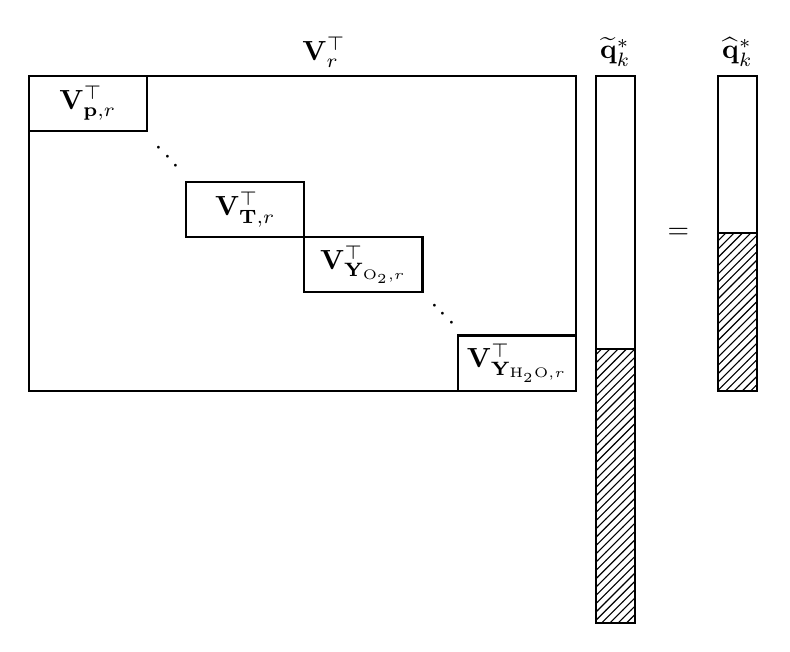
\begin{tikzpicture}[
    wide box/.style={draw, thick, minimum width=1.5cm, minimum height=0.7cm, inner sep=0pt},
    wide big box/.style={draw, thick, minimum width=6.95cm, minimum height=4cm, inner sep=0pt},
    long vec/.style={draw, thick, minimum width=0.5cm, minimum height=6.95cm, inner sep=0pt},
    shaded vec/.style={draw, thick, pattern=north east lines, minimum width=0.5cm, minimum height=3.475cm, inner sep=0pt},
    short vec/.style={draw, thick, minimum width=0.5cm, minimum height=4cm, inner sep=0pt},
    short shaded vec/.style={draw, thick, pattern=north east lines, minimum width=0.5cm, minimum height=2cm, inner sep=0pt}
]

    % Block-structured POD basis
    \draw (3.225, 4) node[wide big box] {};
    
    \draw (0.5, 5.65) node[wide box] {};
    \node at (0.5, 5.65) {$\bV_{\bp, r}^{\top}$};
    \node[rotate=135] at (1.5, 5) {$\cdots$};

    \draw (2.5, 4.3) node[wide box] {};
    \node at (2.5, 4.3) {$\bV_{\bT, r}^{\top}$};

    \draw (4.0, 3.60) node[wide box] {};
    \node at (4.0, 3.60) {$\bV_{\bY_{\textnormal{O}_2, r}}^{\top}$};
    \node[rotate=135] at (5.00, 3.0) {$\cdots$};
    
    \draw (5.95, 2.35) node[wide box] {};
    \node at (5.95, 2.35) {$\bV_{\bY_{\textnormal{H}_2\textnormal{O},r}}^{\top}$};

    \node at (3.5, 6.3) {$\bV_r^\top$};

    % high-dim state
    \draw (7.2, 2.525) node[long vec] {};
    % corrected state
    \draw (7.2, 0.79) node[shaded vec] {};
    
    \node at (7.2, 6.3) {$\widetilde{\bq}_k^*$};

    % Equal sign
    \node at (8.0, 4) {=};

    % low-dim state
    \draw (8.75, 4) node[short vec] {};

    % low-dim corrected state
    \draw (8.75, 3) node[short shaded vec] {};
    
    \node at (8.75, 6.3) {$\widehat{\bq}_k^*$};

\end{tikzpicture}

\caption{Projection of the species-limited high-dimensional state at time step $k$, $\widetilde{\bs}_k^*$, when block-structured POD basis is used.}
\label{fig:block_structured_POD}
\end{figure}



%%%%%%%%%%%%%%%%%%%%%%%%%%%%%%%%%%%%%%%
% BIBLIOGRAPHY
%%%%%%%%%%%%%%%%%%%%%%%%%%%%%%%%%%%%%%%
\bibliography{references}
\bibliographystyle{abbrv}
% \bibliographystyle{unsrt}

\end{document}